\documentclass[12pt]{report}

\usepackage{verbatim}
\usepackage{fullpage}
\usepackage{etoolbox}
\usepackage{lipsum}
\usepackage{graphicx}
\usepackage{hyperref}
\usepackage{titlesec}
\usepackage{pdftexcmds}
\usepackage{minted}
\usepackage{fixltx2e}
\usepackage{calc}
\usepackage{doxygen}
\usepackage[export]{adjustbox} % also loads graphicx
\usepackage{graphicx}
\usepackage[utf8]{inputenc}
\usepackage{makeidx}
\usepackage{multicol}
\usepackage{multirow}
\PassOptionsToPackage{warn}{textcomp}
\usepackage{textcomp}
\usepackage[nointegrals]{wasysym}
\usepackage[table]{xcolor}

% Font selection

\renewcommand{\DoxyLabelFont}{}
\newcommand{\+}{\discretionary{\mbox{\scriptsize$\hookleftarrow$}}{}{}}

% Page & text layout
\usepackage{geometry}



% Headers & footers
\usepackage{fancyhdr}
\renewcommand{\footrulewidth}{0.4pt}
\renewcommand{\chaptermark}[1]{%
  \markboth{#1}{}%
}
\renewcommand{\sectionmark}[1]{%
  \markright{\thesection\ #1}%
}

% Indices & bibliography
\usepackage{natbib}
\usepackage[titles]{tocloft}
\setcounter{tocdepth}{3}
\setcounter{secnumdepth}{5}
\makeindex

% Hyperlinks (required, but should be loaded last)
\usepackage{ifpdf}
\hypersetup{%
  colorlinks=false,%
  linkcolor=blue,%
  citecolor=blue,%
  unicode%
}

% Custom commands
\newcommand{\clearemptydoublepage}{%
  \newpage{\pagestyle{empty}\cleardoublepage}%
}


\graphicspath{ {res/} }
\setcounter{secnumdepth}{4}
\titleformat{\paragraph}
{\normalfont\normalsize\bfseries}{\theparagraph}{1em}{}
\titlespacing*{\paragraph}
{0pt}{3.25ex plus 1ex minus .2ex}{1.5ex plus .2ex}

\newcommand{\HRule}{\rule{\linewidth}{0.5mm}}
\renewcommand\emph{\textbf}
\renewcommand{\baselinestretch}{1.1}

\newcommand{\printSQLtest}[1]
{
    \inputminted[linenos, breaklines, breakbytoken, tabsize=4, fontsize=\footnotesize]{mysql}{#1}
}

\newcommand{\printPHPImpl}[1]
{
    \inputminted[linenos, breaklines, breakbytoken, tabsize=4, fontsize=\footnotesize]{php}{#1}
}

\newcommand{\printPHP}[1]
{
    \printPHP{../www/php/#1}
}

\newcommand{\printSQLTablepage}[2]
{    
    \subsection{#2}
    \subsubsection{Code}
    \printSQLtest{../sql/parts/#1}
    \subsubsection{Explanation}
}

\begin{document}



\begin{titlepage}

    \center

    \textsc{\LARGE Universita' degli Studi di Messina}\\[0.1cm]
    \textsc{\Large Dipartimento di Matematica e Informatica}\\[0.5cm]
    \textsc{\Large Programming II project}\\[0.5cm]

    \HRule \\[0.4cm]
    { \huge \bfseries NetLayer}\\[0.1cm]

    {\large 11 June 2015}
    \HRule \\[1.5cm]

    \begin{minipage}{0.4\textwidth}
    \begin{flushleft} \large
    \emph{Authors:}\\
    Vittorio \textsc{Romeo}
    \end{flushleft}
    \end{minipage}
    ~
    \begin{minipage}{0.4\textwidth}
    \begin{flushright} \large
    \emph{Professors:} \\
    Massimo \textsc{Villari}


    \end{flushright}
    \end{minipage}\\[4cm]

    \vfill


    \begin{minipage}{\linewidth}
        \centering
        \begin{minipage}{0.35\linewidth}
            \begin{figure}[H]
                \center
                
\includegraphics[width=2cm, height=2cm]{logovee}

                \url{http://vittorioromeo.info}
            \end{figure}
        \end{minipage}
        \hspace{0.27\linewidth}
        \begin{minipage}{0.35\linewidth}
            \begin{figure}[H]
                \center
                
\includegraphics[width=2cm, height=2cm]{logounime}

                \url{http://unime.it}
            \end{figure}
        \end{minipage}
    \end{minipage}\\[3cm]
\end{titlepage}



\pagenumbering{gobble}
\newcommand{\atoc}[1]{\addtocontents{toc}{#1\par}}
\renewcommand{\thesection}{\arabic{section}.}
\tableofcontents
\newpage
\pagenumbering{arabic}




\part{Project specifications}

    The following part of the document describes the project and its design/development process without exploring its implementation details.

    The part begins with a synthesis of the \emph{client request}. After a careful analysis of the request, a \emph{Software Requirements Specification} (SRS) was written.

    Writing a correct and informative SRS is of utmost importance to achieve an high-quality final product and ensuring the development process goes smoothly.

    The SRS will cover the following points in depth:

    \begin{itemize}
        \item \emph{Scope and purpose}.
        \item \emph{Feature and functions}.
        \item \emph{External interface requirements}.
        \item \emph{Functional requirements}.
        \item \emph{Example use cases}.
        \item \emph{Non-functional requirements}.
        \item \emph{Analysis models}.
    \end{itemize}

    \chapter{Client request}

        The client requests the design and implementation of an \emph{open-source multi-purpose C++14 networking library}.

        The library must allow the client to develop its own \emph{server-client} architectures and applications with ease, while still being performant and allowing low-level operations if required.

        The client intends to use the library as a basis for the networking layer in applications belonging to different domains, ranging from \emph{chat web applications} to \emph{real-time games and simulations}.

        The library must fulfill the following requirements:

        \begin{itemize}
            \item The library must be written in \emph{modern C++14}, making use of the latest features to improve performance, readability and flexibility.

            \item The library must target \emph{UNIX} systems, \emph{Windows} and \emph{MacOS}.

            \item The library must have a \emph{layered architecture}, allowing developers using it to go as low-level/high-level they desire.

            \item The library must deal with \emph{byte serialization} of native and user-defined classes. Nested serializable data structures must be supported.

            \item The library must provide a generic \emph{tunnel abstraction} that represents a network entity providing and receiving data. A UDP socket tunnel implementation must be provided with the library.

            \item The library must provide an high-level abstraction for \emph{server-client} multithreaded architectures, allowing applications to asynchronously interact with any number of sockets and conveniently handle received packets via function dispatching.

            \item The library must provide metaprogramming facilities to generate and bind packet types at compile-time, allowing performant code generation for serialization/deserialization and communication.

            \item The library must be released under an \emph{open-source} license and promote collaboration and external contributions.
        \end{itemize}

        The client intends using the requested library \emph{to build platforms} for various projects, both for internal company usage and public usage.

        It is imperative for the library to be easily integrable with existing legacy system, such as architectures depending on relational databases.

        For ease of development and deployment, the client requested the library to be optionally usable in \emph{header-only} mode and compatibility with the \emph{CMake} build system.

        The abstraction provided by the library must work asynchronously by default, but an option to use blocking IO must be present.

    \chapter{Software Requirements Specification}


        \section{Introduction}

            \subsection{Software engineering}

                \emph{Software engineering} is the study and an application of engineering to the design, development, and maintenance of software.

                The Bureau of Labor Statistics' definition is Research, design, develop, and test operating systems-level software, compilers, and network distribution software for medical, industrial, military, communications, aerospace, business, scientific, and general computing applications.

                Typical formal definitions of software engineering are:

                \begin{itemize}
                    \item The systematic application of scientific and technological knowledge, methods, and experience to the design, implementation, testing, and documentation of software.
                    \item The application of a systematic, disciplined, quantifiable approach to the development, operation, and maintenance of software.
                    \item An engineering discipline that is concerned with all aspects of software production.
                    \item The establishment and use of sound engineering principles in order to economically obtain software that is reliable and works efficiently on real machines.
                \end{itemize}

                \subsubsection{Background}

                    The term \emph{software engineering} goes back to the '60s, when more complex programs started to be developed by teams composed by experts.

                    There was a radical transformation of software: from \emph{artisan product} to \emph{industrial product}.

                    A software engineer needs to be a good programmer, an algorithm and data structures expert with good knowledge of one or more programming languages.

                    He needs to know various design processes, must have the ability to convert generic requirements in well-detailed and accurate specifications, and needs to be able to communicate with the end-user in a language comprehensible to him comprehensible.

                    Software engineering, is, however, a discipline that's still evolving. There still are no definitive standards for the software development process.

                    Compared to traditional engineering, which is based upon mathematics and solid methods and where well-defined standards need to be followed, software engineering is greatly dependent on personal experience rather than mathematical tools.

                    Here's a brief history of software engineering:

                    \begin{itemize}
                        \item \emph{1950s}: Computers start to be used extensively in business applications.
                        \item \emph{1960s}: The first software product is marketed.

                        IBM announces its unbundling in June 1969.
                        \item \emph{1970s}: Software products are now regularly bought by normal users.

                        The software development industry grows rapidly despite the lack of financing.

                        The first software houses begin to emerge.
                    \end{itemize}

                \subsubsection{Differences with programming}

                    \begin{itemize}
                        \item A programmer writes a complete program.
                        \item A software engineer writes a software component that will be combined with components written by other software engineers to build a system.
                    \end{itemize}

                    \begin{itemize}
                        \item Programming is primarily a personal activity.
                        \item Software engineering is essentially a team activity.
                    \end{itemize}

                    \begin{itemize}
                        \item Programming is just one aspect of software development.
                        \item Large software systems must be developed similar to other engineering practices.
                    \end{itemize}

            \subsection{SRS}

                This \emph{Software Requirements Specification} (SRS) chapter contains all the information needed by software engineers and project managers to design and implement the requested forum creation/management framework.

                The SRS was written following the \emph{Institute of Electrical and Electronics Engineers} (IEEE) guidelines on SRS creation.

            \subsection{Purpose}
                The SRS chapter is contained in the \emph{non-technical} part of the thesis.

                Its purpose is providing a \emph{comprehensive description} of the objective and environment for the software under development.

                The SRS fully describes \emph{what the software will do} and \emph{how it will be expected to perform}.

            \subsection{Scope}

                \subsubsection{Identity}
                    The software that will be designed and produced will be called \emph{NetLayer}.

                \subsubsection{Feature extents}

                    The complete product will:

                    \begin{itemize}
                        \item Provide a library for the \emph{development of multi-purpose network applications and architectures}.
                        \item Provide abstractions for all the major  \emph{operating systems' networking layer}.
                        \item Provide an extensible and flexible  \emph{data serialization} module for primitive and user-defined classes.
                    \end{itemize}

                    NetLayer, however, will not be a complete framework for the development of applications. Every part of an application that does not deal with networking issues will not be covered by the product.

                \subsubsection{Benefits and objectives}

                    Development using NetLayer will give companies and individuals several benefits over \"from-scratch\" development.

                    \begin{itemize}
                        \item Usage of NetLayer will provide access to an \emph{easy-to-integrate} and \emph{easy-to-use} networking library.
                        \item Development and testing time will be \emph{significantly reduced}.
                        \item Code making use of the library will be \emph{modern, efficient and readable} thanks to C++14 features and abstractions.
                    \end{itemize}

        \section{General description}
            \subsection{Product perspective and functions}
                The product shares many basic aspects and features with existing networking libraries, improving upon them in the following ways:

                \begin{itemize}
                    \item A layer-based architecture allows developers to make use of both low-level constructs and operations and high-level abstractions in the same application.
                    \item The library will optionally allow developers to use a programming style similar to \emph{functional programming}, making use of callbacks and first-class functions to deal with packet management and function dispatching.
                    \item
                \end{itemize}

            \subsection{User characteristics}
                NetLayer is targeted towards modern C++ developers experienced with C++11 and C++14 features. The library makes heavy use of modern metaprogramming paradigms and techniques - unfamiliar users will not be able to make full use of the library.

                A \"more functional\" interface is provided where possible, allowing users to use convenient abstractions for data serialization functions and networking functions.

                Familiarity with multithreading and synchronous computation is also required to use the library.

        \section{Glossary}

            The following list contains all the main elements that compose the architecture of NetLayer.

            \begin{itemize}
                \item \emph{Packet Buffer}: dynamically resizable buffer that can store and provide serialized generic data.
                \item \emph{Address}: union of an IP address and a port.
                \item \emph{Payload}: abstraction consisting of an Address and PcktBuf. It can be sent to and received by Tunnel instances.
                \item \emph{Tunnel}: abstraction of a Payload provider/receiver. The default Tunnel is an UDP socket.
                \item \emph{Thread Safe Queue}: a lock-based thread safe queue that supports concurrent enqueueing and dequeueing.
                \item \emph{Managed Packet Buffer}: abstraction consisting of a Thread Safe Queue and a reference to a Tunnel. It can be either a \emph{Managed Receive Buffer}, which enqueues received data from the tunnel, or a \emph{Managed Send Buffer}, which enqueues data that will be sent through the tunnel.
                \item \emph{Managed Host}: union of an Address, a Tunnel, a Managed Receive Buffer and a Managed Send Buffer. Represents a network entity capable of sending and receiving data through a tunnel.
                \item \emph{Serializable}: abstraction over a tuple of generic types that automatically allows the user to serialize and deserialize data. Serializable packets can also be nested and contain dynamically-resizable data structures.
                \item \emph{Packet Bind}: compile-time bind of a Serializable to a Packet type. Used to generate a dispatch table.
                \item \emph{Dispatch Table}: compile-time function table that binds a function to specific packet binds. Used to handle received packets.
                \item \emph{Context Managed Host}: union of a managed host and a dispatch table.
            \end{itemize}

        \section{Specific requirements}

            \subsection{External interface requirements}

                \emph{External interface requirements} identify and document the interfaces to other systems and external entities within the project scope.

                \subsubsection{User interfaces}
                    The product will not provide any graphical user interface. The users of the library will be able to access its functions and types using C++14.

                \subsubsection{Software interfaces}
                    The \emph{open-source policy} of NetLayer will allow its users to expand or improve existing functionality and to interact with other existing technologies.

            \subsection{Functional requirements}
                In software engineering, a \emph{functional requirement} defines a function of a system and its components.

                Functional requirements may be \emph{calculations}, \emph{technical details}, \emph{data manipulation and processing} and other specific functionality that define what a system is supposed to accomplish.

                Behavioral requirements describing all the cases where the system uses the functional requirements are captured in \emph{use cases}.

                \subsubsection{Packet management}
                    \begin{itemize}
                        \item \emph{Payloads and thread-safe queue}: an abstraction consisting of an address and data is provided, along with a thread-safe queue that is used for sending/receiving data to/from the network in managed buffers.
                        \item \emph{Managed buffers}: payloads will be enqueued and dequeued in managed buffers, that allow to asynchronously access the contents of their queue.
                    \end{itemize}

                    
                    \begin{figure}[!htb]
                    \caption{Managed buffer example diagram.}
                    \centering
                    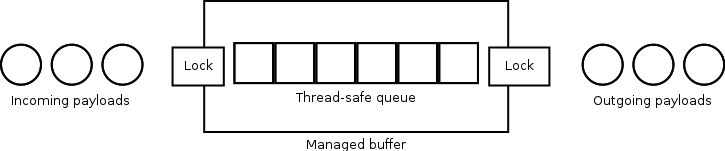
\includegraphics[width=0.85\textwidth]{d/other/managedbuf.png}
                    \end{figure}

                 \subsubsection{Data serialization}
                    \begin{itemize}
                        \item \emph{Fundamental types}: fundamental C++ type serialization will automatically be provided by the library.
                        \item \emph{Common C++ classes}: serialization for commonly used C++ classes, such as \mintinline{cpp}{std::vector} and \mintinline{cpp}{std::array}, is provided by default.
                        \item \emph{Extensible serialization}: library user will be able to extend the serialization system with their own types, using simple class inheritance or macros for convenience.
                    \end{itemize}

                    
                    \begin{figure}[!htb]
                    \caption{Automatic serialization hierarchy.}
                    \centering
                    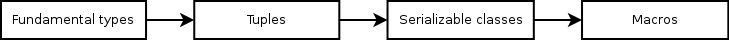
\includegraphics[width=1\textwidth]{d/other/serialization.png}
                    \end{figure}

                  \subsubsection{Tunnel management}
                    \begin{itemize}
                        \item \emph{Default tunnel: UDP}: a tunnel implementation, wrapping an UDP socket, is provided by default.
                        \item \emph{Default tunnel: mock}: a mock tunnel, for unit-testing purposes, is provided by default.
                        \item \emph{Tunnel interface}: an extensible tunnel interface is provided, allowing the users of the library to implement their own network tunnels.
                    \end{itemize}

                    \begin{figure}[!htb]
                    \caption{Tunnel example diagram.}
                    \centering
                    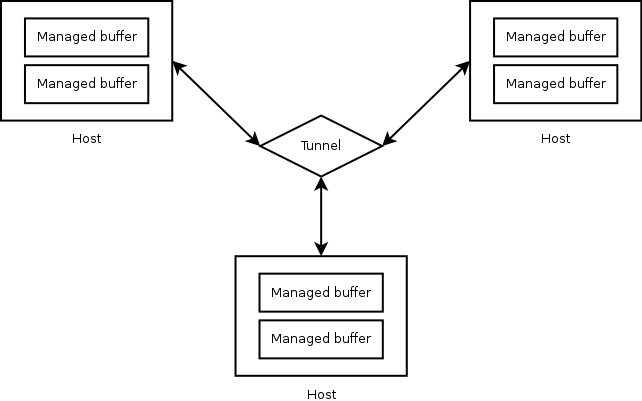
\includegraphics[width=0.85\textwidth]{d/other/tunnel.png}
                    \end{figure}

                \subsubsection{Context binding}
                 \begin{itemize}
                        \item \emph{Managed hosts}: abstraction consisting of a send managed buffer and a receive managed buffer. Allows the user to add processing threads and to poll the buffers for received data.
                        \item \emph{Dispatch table}: an extensible table, configurable at compile-time, is provided to allow the user to define functions which will automatically handle specific packet types.
                        \item \emph{Context host}: union of a managed host and a dispatch table. Provides a convenient interface to quickly develop a server/client architecture capable of sending and receiving payloads.
                    \end{itemize}

                \begin{figure}[!htb]
                    \caption{Context host diagram.}
                    \centering
                    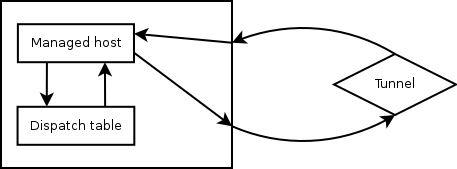
\includegraphics[width=0.85\textwidth]{d/other/ctxhost.png}
                    \end{figure}

            \newpage

            \subsection{Example use cases}
                In software and systems engineering, a \emph{use case} is a list of steps, typically defining interactions between one or more actors and a system, to achieve a goal.

                In the following examples, we'll cover possible use cases for two different developer types using NetLayer:

                \begin{itemize}
                            \item \emph{Networking layer developer}: developer managing packet types, tunnel types and their bindings.
                            \item \emph{Application layer developer}: developer managing application logic, making use of existing NetLayer bindings.
                        \end{itemize}

                \subsubsection{Defining tunnel types}
                    
                    Defining tunnel types is a low-level operation done by networking layer developers. It allows NetLayer users to implement their own protocols or mock payload providers/receivers.

                    \paragraph{Actors}
                        \begin{itemize}
                            \item Networking layer developer.
                            \item NetLayer library.
                        \end{itemize}

                    \paragraph{Pre-conditions}
                        \begin{itemize}
                            \item NetLayer was correctly included.
                        \end{itemize}

                    \paragraph{Post-conditions}
                        \begin{itemize}
                            \item An usable tunnel type for context hosts or manual payload management was defined.
                        \end{itemize}

                    \begin{figure}[H]
                    \caption{Defining tunnel types - use case diagram.}
                    \centering
                    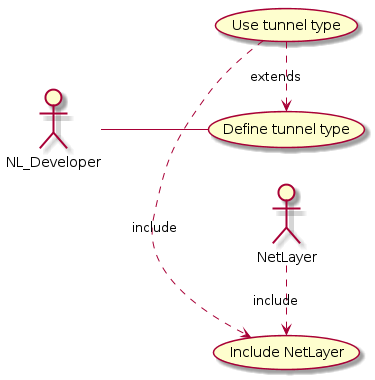
\includegraphics[width=0.65\textwidth]{d/uc/def_tunnels.png}
                    \end{figure}

                \subsubsection{Defining serializable types}
                    
                    Serializable types will be usually defined by networking layer developers and used by both types of developers. 
                    Fundamental types are automatically serializable. Tuples of fundamental types can be marked as serializable and wrapped in custom interfaces using either compile-time inheritance or helper preprocessor macros.

                    \paragraph{Actors}
                        \begin{itemize}
                            \item Networking layer developer.
                            \item Application layer developer.
                            \item NetLayer library.
                        \end{itemize}

                    \paragraph{Pre-conditions}
                        \begin{itemize}
                            \item NetLayer was correctly included.
                        \end{itemize}

                    \paragraph{Post-conditions}
                        \begin{itemize}
                            \item Any number of serializable types were defined.
                            \item Defined types can be sent/received through tunnels.
                            \item Defined types can be used as normal C++ types.
                        \end{itemize}

                    \begin{figure}[H]
                    \caption{Defining serializable types - use case diagram.}
                    \centering
                    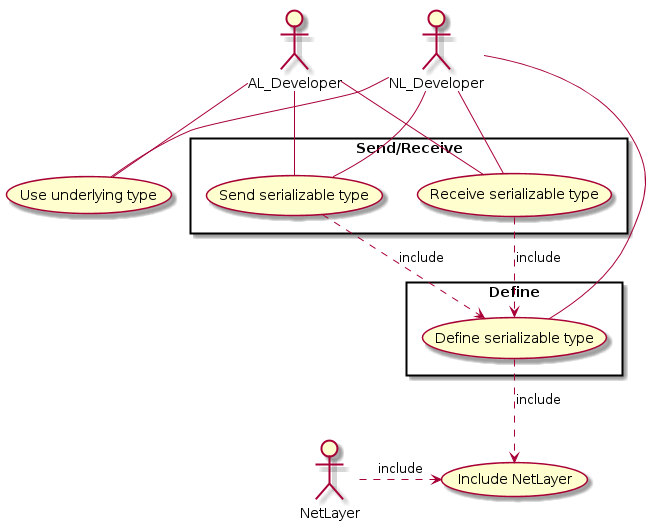
\includegraphics[width=0.65\textwidth]{d/uc/def_serializable_t.png}
                    \end{figure}


                \subsubsection{Binding types to dispatch table}
                    
                    The creation and management of a dispatch table is usually handled by networking layer developers. They will define and bind all packet types that can be received and sent by the application.

                    \paragraph{Actors}
                        \begin{itemize}
                            \item Networking layer developer.
                            \item NetLayer library.
                        \end{itemize}

                    \paragraph{Pre-conditions}
                        \begin{itemize}
                            \item NetLayer was correctly included.
                        \end{itemize}

                    \paragraph{Post-conditions}
                        \begin{itemize}
                            \item A dispatch table was defined.
                            \item Functions can now be assigned to every inbound payload type.
                        \end{itemize}

                    \begin{figure}[H]
                    \caption{Binding types to dispatch table - use case diagram.}
                    \centering
                    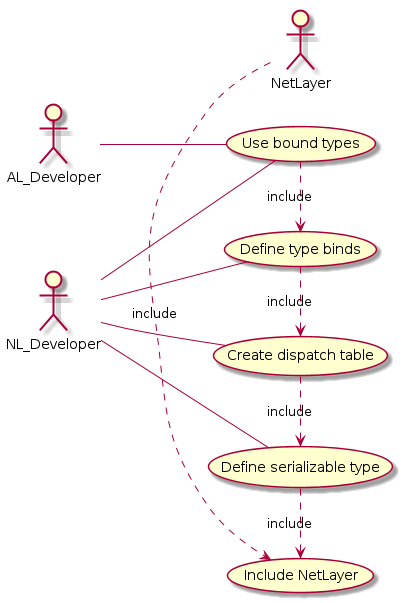
\includegraphics[width=0.65\textwidth]{d/uc/bind_types.png}
                    \end{figure}


                \subsubsection{Defining a context host}
                    
                    After the creation of a dispatch table, the definition of a context host is required. A context host is the union of a dispatch table and a managed host.

                    \paragraph{Actors}
                        \begin{itemize}
                            \item Networking layer developer.
                            \item NetLayer library.
                        \end{itemize}

                     \paragraph{Pre-conditions}
                        \begin{itemize}
                            \item NetLayer was correctly included.
                            \item A dispatch table was created.
                            \item A tunnel type was chosen.
                        \end{itemize}

                    \paragraph{Post-conditions}
                        \begin{itemize}
                            \item An usable context host was defined.
                            \item A previously defined dispatch table is now bound to the context host.
                            \item The context host can now send/receive bound payload types.
                        \end{itemize}

                    \begin{figure}[H]
                    \caption{Defining a context host - use case diagram.}
                    \centering
                    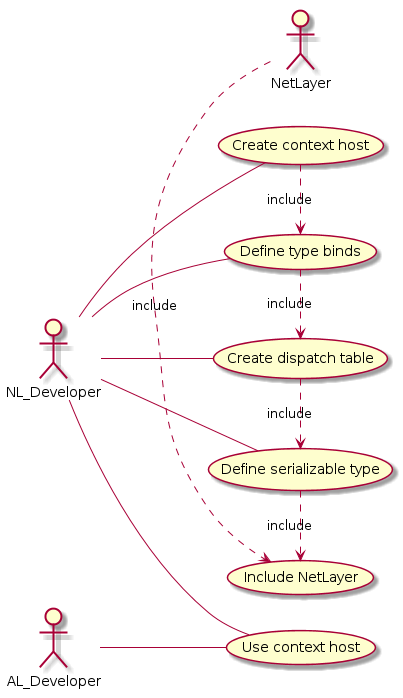
\includegraphics[width=0.65\textwidth]{d/uc/def_context_host.png}
                    \end{figure}


                \subsubsection{Handling incoming payloads}
                    
                    Incoming payloads can be either handled by managed hosts, bypassing the dispatch table, or by context hosts. 
                    Context hosts automatically call a bound function depending on the type of the received payload.

                    \paragraph{Actors}
                        \begin{itemize}
                            \item Networking layer developer.
                            \item Application layer developer.
                            \item NetLayer library.
                        \end{itemize}

                    \paragraph{Pre-conditions}
                        \begin{itemize}
                            \item NetLayer was correctly included.
                            \item A context host was defined.
                            \item Payload types were bound to dispatch table.
                        \end{itemize}

                    \paragraph{Flow of events}
                        \begin{itemize}
                            \item
                        \end{itemize}

                    \paragraph{Post-conditions}
                        \begin{itemize}
                            \item Incoming payloads were handled or an error occurred.
                        \end{itemize}

                    \begin{figure}[H]
                    \caption{Handling incoming payloads - use case diagram.}
                    \centering
                    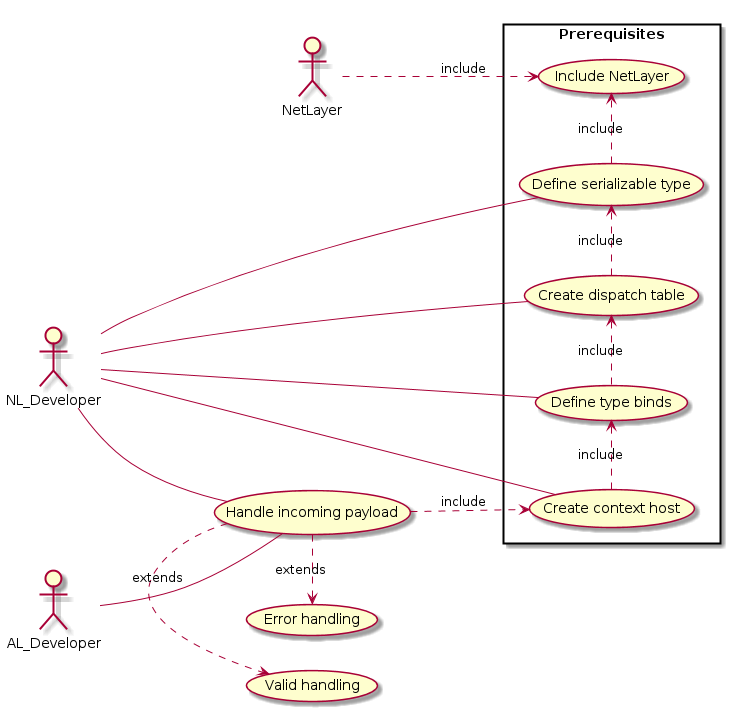
\includegraphics[width=0.65\textwidth]{d/uc/inc_payloads.png}
                    \end{figure}



                \subsubsection{Handling outgoing payloads}
                    
                    Outgoing packets can be sent both by managed hosts and context hosts. Context hosts provide functionality to mark the type of the packet, so that receivers can handle it thanks to dispatch tables.

                    \paragraph{Actors}
                        \begin{itemize}
                            \item Networking layer developer.
                            \item Application layer developer.
                            \item NetLayer library.
                        \end{itemize}

                    \paragraph{Pre-conditions}
                        \begin{itemize}
                            \item NetLayer was correctly included.
                            \item A context host was defined.
                            \item Payload types were bound to dispatch table.
                        \end{itemize}

                    \paragraph{Post-conditions}
                        \begin{itemize}
                            \item Outgoing payloads were sent or an error occurred.
                        \end{itemize}

                    \begin{figure}[H]
                    \caption{Handling outgoing payloads - use case diagram.}
                    \centering
                    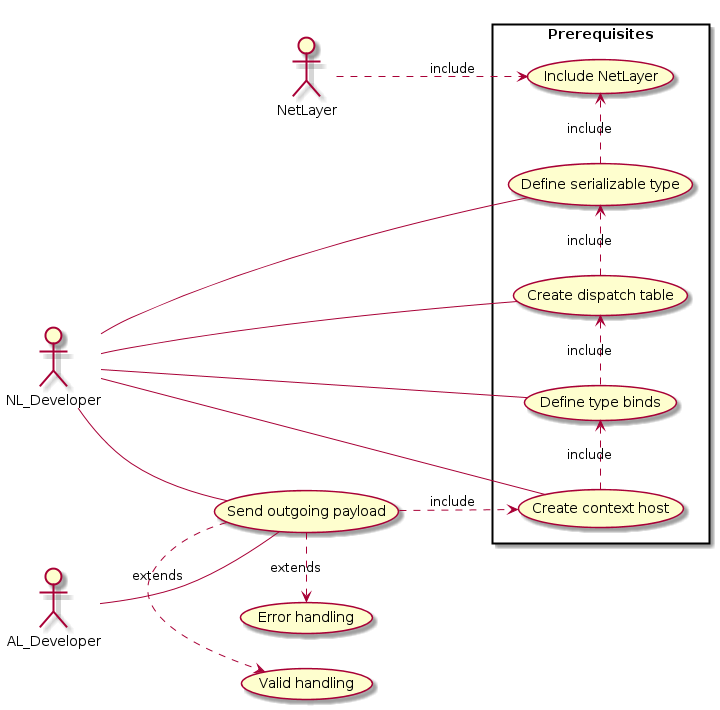
\includegraphics[width=0.65\textwidth]{d/uc/outgoing.png}
                    \end{figure}



            \newpage

            \subsection{Non-functional requirements}
                Functional requirements are supported by \emph{non-functional requirements} (also known as quality requirements), which impose constraints on the design or implementation (such as performance requirements, security, or reliability).

                \subsubsection{Performance}
                    The system will be designed from the ground-up with emphasis on performance. 

                    The layered architecture will allow users to follow the \emph{pay only what you use} principle, which is one of C++'s biggest selling points.

                    NetLayer tries to do as much as possible during compilation, avoiding unnecessary run-time polymorphism overhead.

                \subsubsection{Reliability}
                    The system will have to be reliable and keep working in case of errors.

                    Since NetLayer is a general-purpose library, intended for use in multiple domains, \emph{exceptions are not used} throughout the library. 
                    Real-time simulation and game development industries prefer avoiding using exceptions because they unfortunately always bring a small amount of runtime overhead, even when rarely used throughout the program.

                    NetLayer will allow users to define and use their preferred error handling systems.

                \subsubsection{Security}

                    Encryption and other security features are out of NetLayer's scope - users can implement them on top of the library if necessary.

                \subsubsection{Maintainability and portability}
                    Being an open-source project, \emph{maintainability}, \emph{extensibility} and \emph{portability} are key.

                    The code layer will be carefully designed and organized to allow easy maintenance, bugfixing and feature addition.

                    To ensure maximum portability, the product will be designed to work on the most popular \emph{GNU/Linux} distributions and will be thoroughly tested on different platforms.

        \section{Analysis models}
            \subsection{Activity diagrams}
                Activity diagrams are graphical representations of workflows of stepwise activities and actions with support for choice, iteration and concurrency.
                In the Unified Modeling Language, activity diagrams are intended to model both computational and organisational processes (i.e. workflows).
                Activity diagrams show the overall flow of control.

                \newpage
                The following diagram shows the required steps to define a serializable type.

                \begin{figure}[H]
                %\caption{}
                \centering
                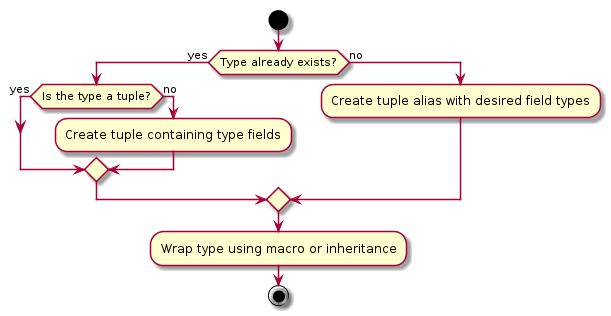
\includegraphics[width=0.7\textwidth]{d/ac/def_ser.png}
                \end{figure}



                \newpage
                The following diagram shows the required steps to serialize an object into a payload.

                \begin{figure}[H]
                %\caption{}
                \centering
                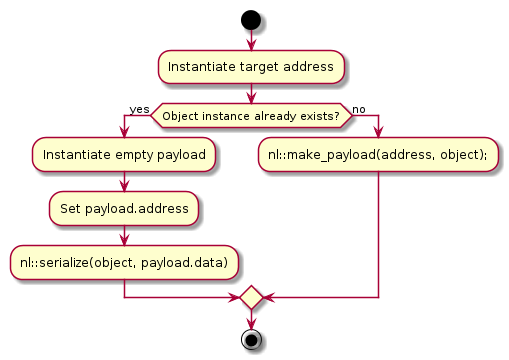
\includegraphics[width=0.7\textwidth]{d/ac/def_ser_obj.png}
                \end{figure}





                \newpage
                The following diagram shows the required steps to deserialize a payload into an object.

                \begin{figure}[H]
                %\caption{}
                \centering
                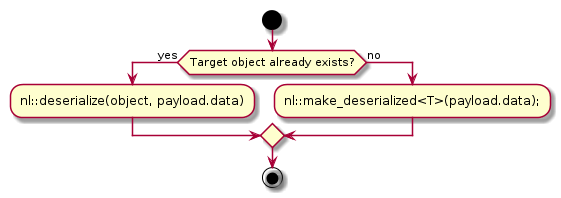
\includegraphics[width=0.7\textwidth]{d/ac/def_deserialize_obj.png}
                \end{figure}





                \newpage
                The following diagram shows the required steps to define a tunnel.

                \begin{figure}[H]
                %\caption{}
                \centering
                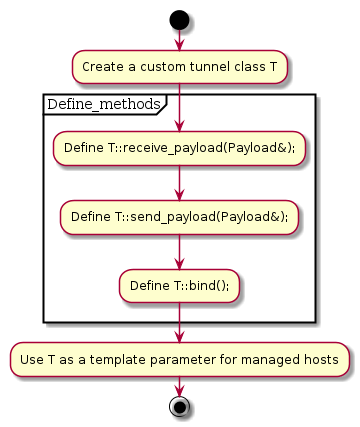
\includegraphics[width=0.7\textwidth]{d/ac/def_tunnel.png}
                \end{figure}






                \newpage
                The following diagram shows the required steps to create a managed host.

                \begin{figure}[H]
                %\caption{}
                \centering
                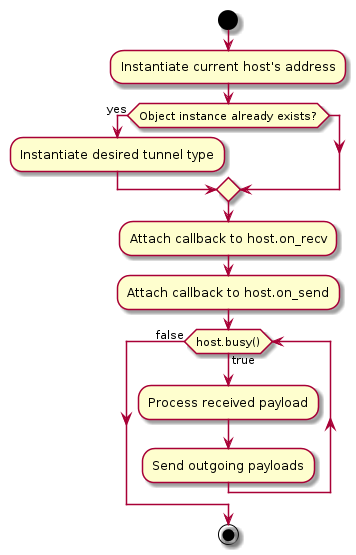
\includegraphics[width=0.7\textwidth]{d/ac/def_manhost.png}
                \end{figure}





                \newpage
                The following diagram shows the required steps to create and bind a dispatch table.

                \begin{figure}[H]
                %\caption{}
                \centering
                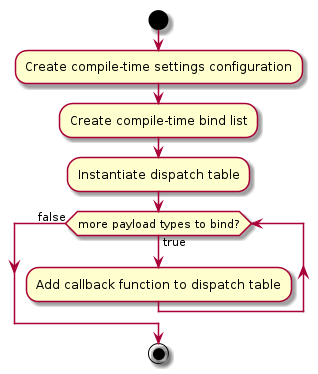
\includegraphics[width=0.7\textwidth]{d/ac/disptable.png}
                \end{figure}





                \newpage
                The following diagram shows the required steps to create a context host.

                \begin{figure}[H]
                %\caption{}
                \centering
                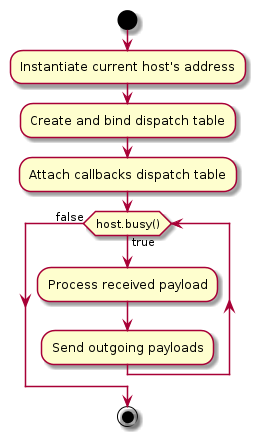
\includegraphics[width=0.7\textwidth]{d/ac/conthost.png}
                \end{figure}





                \newpage
                The following diagram shows the required steps to receive a bound payload.

                \begin{figure}[H]
                %\caption{}
                \centering
                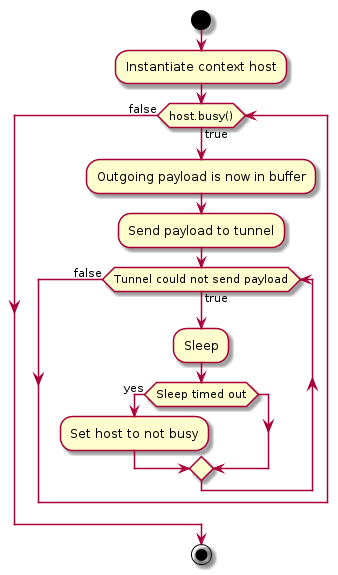
\includegraphics[width=0.7\textwidth]{d/ac/send_p.png}
                \end{figure}





                \newpage
                The following diagram shows the required steps to send a bound payload.

                \begin{figure}[H]
                %\caption{}
                \centering
                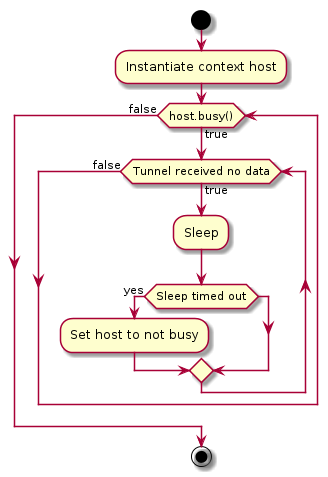
\includegraphics[width=0.7\textwidth]{d/ac/recv_p.png}
                \end{figure}





                \newpage
                \newpage

            \subsection{Class diagrams}

                \emph{Class diagrams} are created using UML.

                The \emph{Unified Modeling Language} (UML) is a general-purpose modeling language in the field of software engineering, which is designed to provide a standard way to visualize the design of a system.

                It offers a way to visualize a system's architectural blueprints in a diagram, including elements such as:

                \begin{itemize}
                    \item Any activities (jobs).
                    \item Individual components of the system.
                    \item And how they can interact with other software components.
                    \item How the system will run.
                    \item How entities interact with others (components and interfaces).
                    \item External user interface.
                \end{itemize}

                \begin{figure}[H]
                \caption{NetLayer complete class diagram.}
                \centering
                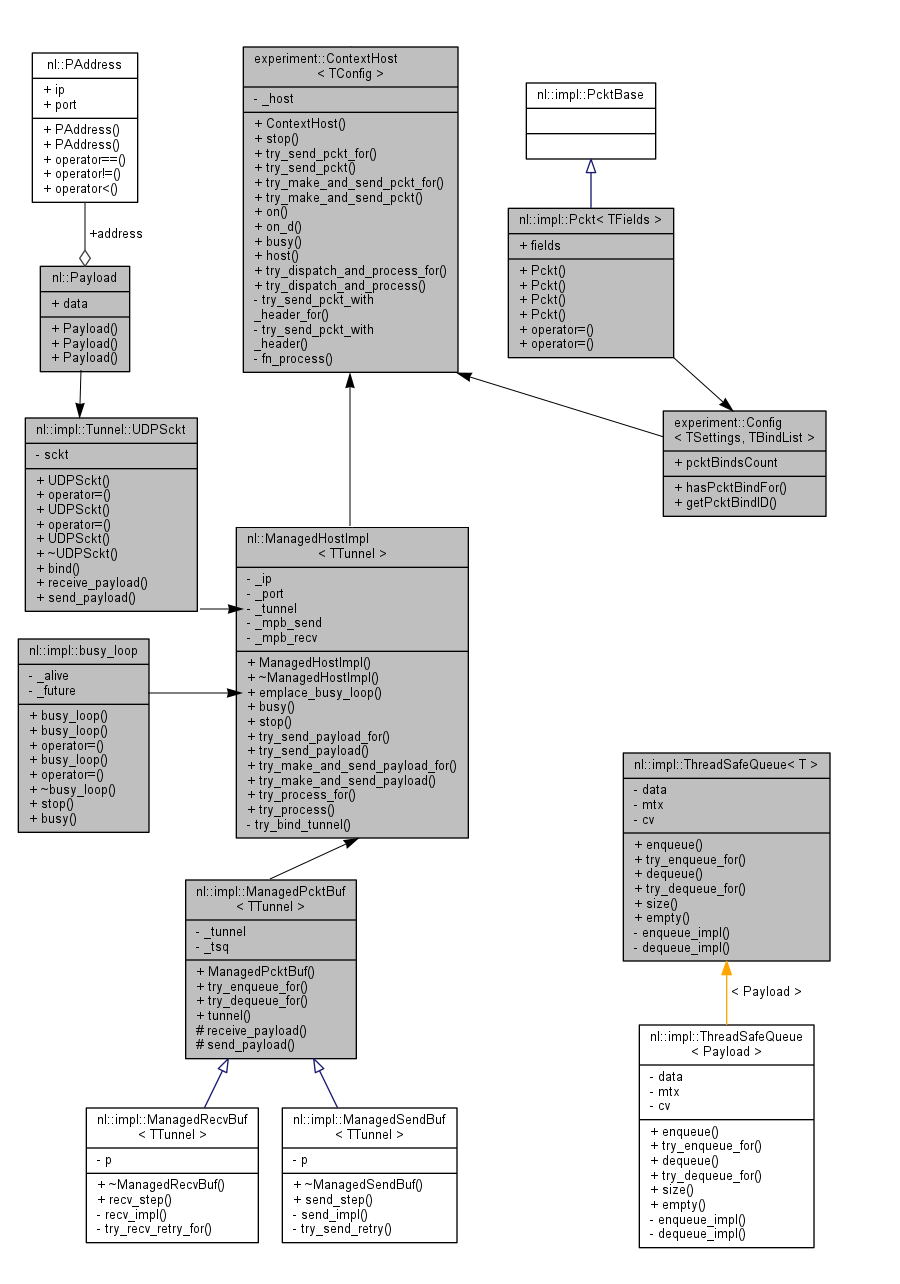
\includegraphics[width=0.9\textwidth]{d/coll/src.png}
                \end{figure}

                \newpage

                \begin{figure}[H]
                \caption{Managed buffer collaboration diagram.}
                \centering
                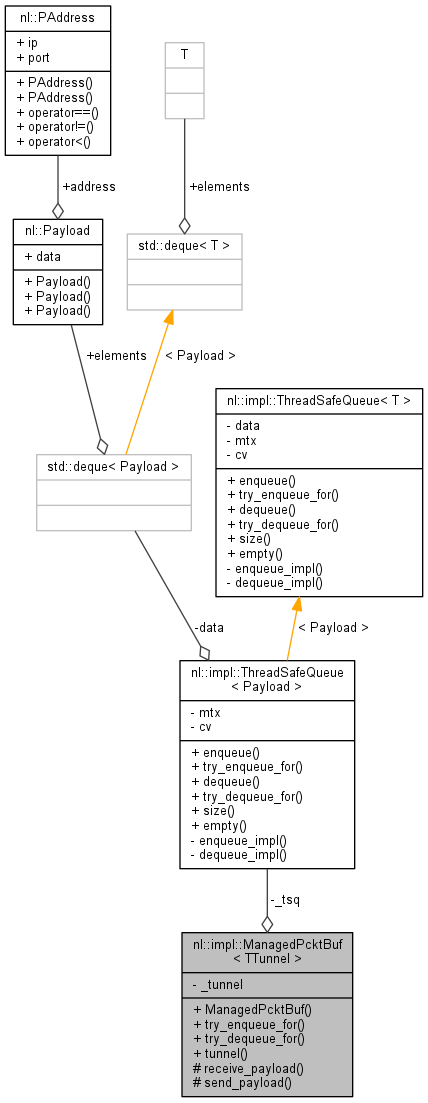
\includegraphics[width=0.4\textwidth]{d/coll/coll_pcktbuf.png}
                \end{figure}

                \newpage

                \begin{figure}[H]
                \caption{Managed host collaboration diagram.}
                \centering
                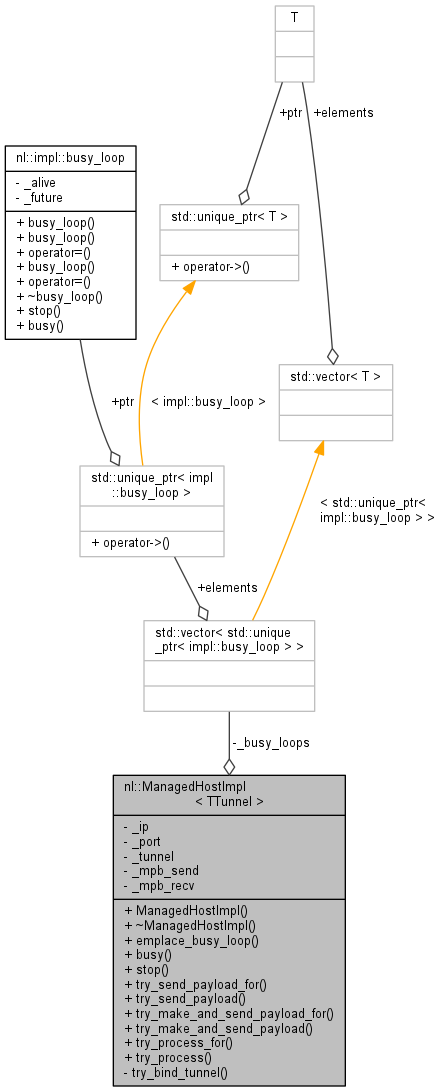
\includegraphics[width=0.4\textwidth]{d/coll/coll_manhost.png}
                \end{figure}

                \newpage

                \begin{figure}[H]
                \caption{Context host collaboration diagram.}
                \centering
                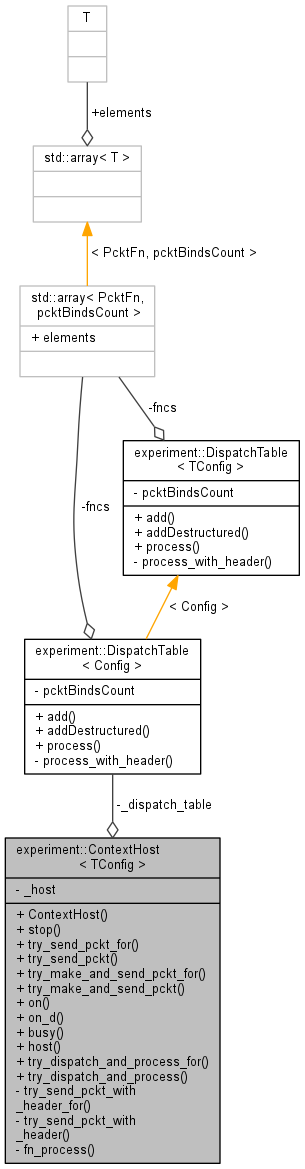
\includegraphics[width=0.4\textwidth]{d/coll/coll_ctxhost.png}
                \end{figure}

                \newpage

                \begin{figure}[H]
                \caption{Dispatch table collaboration diagram.}
                \centering
                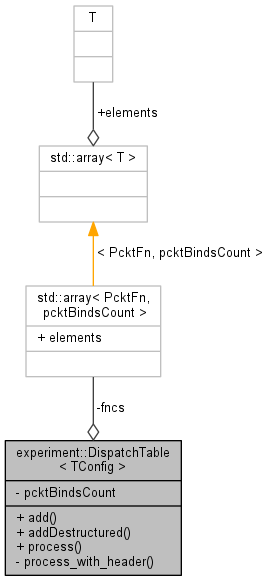
\includegraphics[width=0.4\textwidth]{d/coll/coll_disptab.png}
                \end{figure}

                \newpage                




\part{Technical analysis}
        The following part of the thesis will cover all implementation choices and details for NetLayer in depth.

        Firstly, the \emph{development environment and tools} and \emph{chosen technologies} will be described and motivated.

        Afterwards, the technical details, including code examples and APIs, will be described for the two modules of the application: the \emph{database} and the \emph{web application}.

        Every \emph{table} of the database will be analyzed in detail, directly showing commented \emph{DDL} code. The database also contains important \emph{stored procedures} and \emph{triggers} that are core part of the system's logic and that need to be explained in depth - the related \emph{DML} code will be shown and commented.

        The web application itself is divided in multiple modules:
        \begin{itemize}
            \item A \emph{database interface backend module}, that interfaces with the database and wraps its tables and stored procedures.
            \item A \emph{HTML5 generation module}, that greatly simplifies the creation of dynamic forum web pages by wrapping HTML5 controls in \emph{object-oriented wrappers} that can be easily bound to callbacks and database events.
            \item A \emph{modern responsive AJAX frontend} that allows users and interact with the backend module from multiple device, limiting postbacks and page refreshes.
        \end{itemize}

        \chapter{Development process}

            \section{Environment and tools}
                All modules of veeForum have been developed on \emph{Arch Linux x64}, a lightweight GNU/Linux distribution.

                Arch is installed as a minimal base system, configured by the user upon which their own ideal environment is assembled by installing only what is required or desired for their unique purposes. GUI configuration utilities are not officially provided, and most system configuration is performed from the shell and a text editor. Based on a rolling-release model, Arch strives to stay bleeding edge, and typically offers the latest stable versions of most software.

                No particular integrated development environments (IDEs) were used during the development - a modern graphical text editor, \emph{Sublime Text 3}, was used instead.

            \section{Docker}
                Docker is an open-source project that \emph{automates the deployment of applications} inside software containers, by providing an additional layer of abstraction and automation of operating-system-level virtualization on Linux.

                Docker uses resource isolation features of the Linux kernel such as \emph{cgroups} and \emph{kernel namespaces} to allow independent containers to run within a single Linux instance.

                This technology has been used since the beginning of the development process to \emph{separate veeForum data and packages} from the host system and to dramatically increase \emph{portability} and \emph{ease of testing}.

                Docker is also used for the installation of the product on target systems - with a single command it is possible to \emph{retrieve all required dependencies}, correctly \emph{configure the system} and \emph{automatically install veeForum}.

            \section{Version control system}
                Version control systems (VCSs) allow the \emph{management of changes} to documents, computer programs, large web sites, and other collections of information.

                Nowadays, a version control system is \emph{essential} for the development of any project.
                Being able to track changes, develop features in separate \emph{branches}, have multiple programmers work on the same code base without conflicts and much more is extremely important for projects of any scope and size.

                The chosen VCS is \emph{Git}, a distributed revision control system with an emphasis on \emph{speed}, \emph{data integrity}, and support for \emph{distributed, non-linear workflows}.

                Git is widely appreciated in the private and open-source programming communities - it was initially designed and developed by \emph{Linus Torvalds} for Linux kernel development in 2005, and has since become the most widely adopted version control system for software development.

                The veeForum project is \emph{open-source} and \emph{appreciates feedback and contributions}. It is hosted on \emph{GitHub}, a web-based Git repository hosting service, which offers all of the distributed revision control and source code management (SCM) functionality of Git, while adding \emph{additional features} that make collaboration and public contributions easy and accessible.

            \section{LAMP stack}
                The server and web application run on a \emph{LAMP stack}, on a GNU/Linux machine.

                A LAMP stack is composed by the following technologies:

                \begin{itemize}
                    \item \emph{L}: GNU/Linux machine.
                    \item \emph{A}: Apache HTTP server.

                     The Apache HTTP server is the world's most widely used web server software.

                     Apache has been under open-source development for about 20 years - it supports all modern server-side technologies and programming languages, and also is \emph{extremely reliable} and \emph{secure}.

                    \item \emph{M}: Stands for MySQL server, but \emph{MariaDB}, a modern drop-in replacement for MySQL is used as the DBMS. 

                    MariaDB is fully compliant with the MySQL standard and language, but it is more performant and has additional features. It is the default DBMS in the Arch Linux distribution.

                    By default, MariaDB uses the \emph{XtraDB} storage engine, a performance enhanced fork of the InnoDB storage engine.

                    Percona XtraDB includes all of InnoDB's robust, reliable ACID-compliant design and advanced MVCC architecture, and builds on that solid foundation with more features, more tunability, more metrics, and more scalability. In particular, it is designed to scale better on many cores, to use memory more efficiently, and to be more convenient and useful. 

                    \item \emph{P}: PHP5, the server backend language. 

                    HTML5, PHP5 and JavaScript conformant to the 5.1 ECMAScript specification (along with the JQuery library) are used for the development of the web application. 

                    The \emph{AJAX} (Asynchronous JavaScript and XML) paradigm will be used to ensure that the application feels responsive and that user interaction is immediately reflected on the web application.

                \end{itemize}
               
            \section{Thesis}
                The current document was written using \LaTeX{}, an high-quality typesetting system; it includes features designed for the production of \emph{technical and scientific documentation}.

                \LaTeX{} was chosen for the current document because of the visually pleasant typography, its extensibility features and its abilities to include and highlight source code.

                \subsection{LatexPP}
                    A small \emph{C++14} \LaTeX{} preprocessor named \emph{LatexPP} was developed for the composition of this thesis.

                    LatexPP allows to use an intuitive syntax that avoids markup repetition for code highlighting and macros.

                    Preprocessing and compiling a \LaTeX{} document using LatexPP is simple and can be automated using a simple \emph{bash} script.

\begin{minted}[mathescape, linenos, numbersep=5pt, gobble=2, frame=lines, framesep=2mm, fontsize=\footnotesize]{bash}
    #!/bin/bash

    latexpp ./thesis.lpp > ./thesis.tex
    pdflatex -shell-escape ./thesis.tex && chromium ./thesis.pdf
\end{minted}

                    LatexPP is available as an open-source project on GitHub:

                    \url{https://github.com/SuperV1234/Experiments/Random}


        \chapter{Project structure}
            The project folder and file structure is organized as such:

            \begin{itemize}
                \item \emph{./doc/}

                    Folder containing the documentation of the project.
                    \begin{itemize}
                        \item \emph{./latex/}

                        LatexPP and \LaTeX{}  source and output files.
                    \end{itemize}

                \item \emph{./sql/}

                    Folder containing the SQL DDL scripts.
                    \begin{itemize}
                        \item \emph{./scripts/}

                        Contains all the parts that make up the complete SQL initialization script.

                        \item \emph{./mkScript.sh}

                        Builds the complete SQL initialization scripts from the files in ./scripts/.

                        \item \emph{./script.sql}

                        Complete SQL initialization scripts that sets up a database suitable veeForum.
                    \end{itemize}

                \item \emph{./exe/}

                    Folder containing executable scripts to setup the system.
                    \begin{itemize}
                        \item \emph{./docker/}

                        Docker-related scripts.
                        \begin{itemize}
                            \item \emph{./start.sh}

                            Starts a Docker instance containing veeForum.

                            \item \emph{./cleanup.sh}

                            Cleans any running veeForum Docker instance.

                            \item \emph{./shell.sh}

                            Starts a Docker instance containing veeForum, controlling an instance of bash inside it.

                            \item \emph{./httpdLog.sh}

                            Prints the Apache error log of the current running veeForum Docker instance.
                        \end{itemize}

                    \end{itemize}

                \item \emph{./www/}

                    Folder containing web application data.
                    \begin{itemize}

                        \item \emph{./css/}

                        CSS3 stylesheets.

                        \item \emph{./js/}

                        ECMAScript 5 script files.

                        \item \emph{./json/}

                        Non-relational data storage files, in JSON format.

                        \item \emph{./php/}

                        PHP backend code.
                        \begin{itemize}
                            \item \emph{./lib/}

                            Backend to database interface library and HTML5 generation library.

                            \item \emph{./core/}

                            PHP frontend files that generate the responsive HTML5 web application user interface.
                        \end{itemize}

                    \end{itemize}

            \end{itemize}

 %       \chapter{Hierarchical Index}
%\section{Class Hierarchy}
This inheritance list is sorted roughly, but not completely, alphabetically\+:\begin{DoxyCompactList}
\item \contentsline{section}{nl\+:\+:impl\+:\+:busy\+\_\+loop}{\pageref{classnl_1_1impl_1_1busy__loop}}{}
\item \contentsline{section}{experiment\+:\+:Config$<$ T\+Settings, T\+Bind\+List $>$}{\pageref{structexperiment_1_1Config}}{}
\item \contentsline{section}{experiment\+:\+:Context\+Host$<$ T\+Config $>$}{\pageref{classexperiment_1_1ContextHost}}{}
\item \contentsline{section}{experiment\+:\+:Dispatch\+Table$<$ T\+Config $>$}{\pageref{classexperiment_1_1DispatchTable}}{}
\item \contentsline{section}{experiment\+:\+:Dispatch\+Table$<$ Config $>$}{\pageref{classexperiment_1_1DispatchTable}}{}
\item \contentsline{section}{nl\+:\+:impl\+:\+:Tunnel\+:\+:Fake}{\pageref{structnl_1_1impl_1_1Tunnel_1_1Fake}}{}
\item \contentsline{section}{nl\+:\+:init\+\_\+fields}{\pageref{structnl_1_1init__fields}}{}
\item \contentsline{section}{nl\+:\+:Managed\+Host\+Impl$<$ T\+Tunnel $>$}{\pageref{classnl_1_1ManagedHostImpl}}{}
\item \contentsline{section}{nl\+:\+:impl\+:\+:Managed\+Pckt\+Buf$<$ T\+Tunnel $>$}{\pageref{classnl_1_1impl_1_1ManagedPcktBuf}}{}
\begin{DoxyCompactList}
\item \contentsline{section}{nl\+:\+:impl\+:\+:Managed\+Recv\+Buf$<$ T\+Tunnel $>$}{\pageref{classnl_1_1impl_1_1ManagedRecvBuf}}{}
\item \contentsline{section}{nl\+:\+:impl\+:\+:Managed\+Send\+Buf$<$ T\+Tunnel $>$}{\pageref{classnl_1_1impl_1_1ManagedSendBuf}}{}
\end{DoxyCompactList}
\item \contentsline{section}{nl\+:\+:P\+Address}{\pageref{structnl_1_1PAddress}}{}
\item \contentsline{section}{nl\+:\+:Payload}{\pageref{structnl_1_1Payload}}{}
\item \contentsline{section}{experiment\+:\+:impl\+:\+:pckt\+\_\+bind\+\_\+type$<$ T $>$}{\pageref{structexperiment_1_1impl_1_1pckt__bind__type}}{}
\item \contentsline{section}{nl\+:\+:impl\+:\+:Pckt\+Base}{\pageref{structnl_1_1impl_1_1PcktBase}}{}
\begin{DoxyCompactList}
\item \contentsline{section}{nl\+:\+:impl\+:\+:Pckt$<$ T\+Fields $>$}{\pageref{structnl_1_1impl_1_1Pckt}}{}
\end{DoxyCompactList}
\item \contentsline{section}{experiment\+:\+:Settings$<$ T\+I\+D\+Type $>$}{\pageref{structexperiment_1_1Settings}}{}
\item \contentsline{section}{nl\+:\+:impl\+:\+:Thread\+Safe\+Queue$<$ T $>$}{\pageref{classnl_1_1impl_1_1ThreadSafeQueue}}{}
\item \contentsline{section}{nl\+:\+:impl\+:\+:Thread\+Safe\+Queue$<$ Payload $>$}{\pageref{classnl_1_1impl_1_1ThreadSafeQueue}}{}
\item \contentsline{section}{nl\+:\+:impl\+:\+:Tunnel\+:\+:U\+D\+P\+Sckt}{\pageref{classnl_1_1impl_1_1Tunnel_1_1UDPSckt}}{}
\end{DoxyCompactList}

%\chapter{Class Index}
%\section{Class List}
Here are the classes, structs, unions and interfaces with brief descriptions\+:\begin{DoxyCompactList}
\item\contentsline{section}{\hyperlink{classnl_1_1impl_1_1busy__loop}{nl\+::impl\+::busy\+\_\+loop} \\*Wrapper around an {\ttfamily std\+::future$<$void$>$} that runs a busy loop until explicitly stopped by the user }{\pageref{d5/db9/classnl_1_1impl_1_1busy__loop}}{}
\item\contentsline{section}{\hyperlink{structexperiment_1_1Config}{experiment\+::\+Config$<$ T\+Settings, T\+Bind\+List $>$} }{\pageref{da/d11/structexperiment_1_1Config}}{}
\item\contentsline{section}{\hyperlink{classexperiment_1_1ContextHost}{experiment\+::\+Context\+Host$<$ T\+Config $>$} }{\pageref{de/d57/classexperiment_1_1ContextHost}}{}
\item\contentsline{section}{\hyperlink{classexperiment_1_1DispatchTable}{experiment\+::\+Dispatch\+Table$<$ T\+Config $>$} }{\pageref{db/d90/classexperiment_1_1DispatchTable}}{}
\item\contentsline{section}{\hyperlink{structnl_1_1impl_1_1Tunnel_1_1Fake}{nl\+::impl\+::\+Tunnel\+::\+Fake} }{\pageref{db/dba/structnl_1_1impl_1_1Tunnel_1_1Fake}}{}
\item\contentsline{section}{\hyperlink{structnl_1_1init__fields}{nl\+::init\+\_\+fields} }{\pageref{df/d24/structnl_1_1init__fields}}{}
\item\contentsline{section}{\hyperlink{classnl_1_1ManagedHostImpl}{nl\+::\+Managed\+Host\+Impl$<$ T\+Tunnel $>$} }{\pageref{d3/db6/classnl_1_1ManagedHostImpl}}{}
\item\contentsline{section}{\hyperlink{classnl_1_1impl_1_1ManagedPcktBuf}{nl\+::impl\+::\+Managed\+Pckt\+Buf$<$ T\+Tunnel $>$} }{\pageref{df/dda/classnl_1_1impl_1_1ManagedPcktBuf}}{}
\item\contentsline{section}{\hyperlink{classnl_1_1impl_1_1ManagedRecvBuf}{nl\+::impl\+::\+Managed\+Recv\+Buf$<$ T\+Tunnel $>$} }{\pageref{de/d06/classnl_1_1impl_1_1ManagedRecvBuf}}{}
\item\contentsline{section}{\hyperlink{classnl_1_1impl_1_1ManagedSendBuf}{nl\+::impl\+::\+Managed\+Send\+Buf$<$ T\+Tunnel $>$} }{\pageref{d7/dca/classnl_1_1impl_1_1ManagedSendBuf}}{}
\item\contentsline{section}{\hyperlink{structnl_1_1PAddress}{nl\+::\+P\+Address} }{\pageref{db/dc7/structnl_1_1PAddress}}{}
\item\contentsline{section}{\hyperlink{structnl_1_1Payload}{nl\+::\+Payload} }{\pageref{d4/d26/structnl_1_1Payload}}{}
\item\contentsline{section}{\hyperlink{structnl_1_1impl_1_1Pckt}{nl\+::impl\+::\+Pckt$<$ T\+Fields $>$} }{\pageref{df/da7/structnl_1_1impl_1_1Pckt}}{}
\item\contentsline{section}{\hyperlink{structexperiment_1_1impl_1_1pckt__bind__type}{experiment\+::impl\+::pckt\+\_\+bind\+\_\+type$<$ T $>$} }{\pageref{d9/df3/structexperiment_1_1impl_1_1pckt__bind__type}}{}
\item\contentsline{section}{\hyperlink{structnl_1_1impl_1_1PcktBase}{nl\+::impl\+::\+Pckt\+Base} }{\pageref{dc/d5a/structnl_1_1impl_1_1PcktBase}}{}
\item\contentsline{section}{\hyperlink{structexperiment_1_1Settings}{experiment\+::\+Settings$<$ T\+I\+D\+Type $>$} }{\pageref{dc/d22/structexperiment_1_1Settings}}{}
\item\contentsline{section}{\hyperlink{classnl_1_1impl_1_1ThreadSafeQueue}{nl\+::impl\+::\+Thread\+Safe\+Queue$<$ T $>$} }{\pageref{da/d3d/classnl_1_1impl_1_1ThreadSafeQueue}}{}
\item\contentsline{section}{\hyperlink{classnl_1_1impl_1_1Tunnel_1_1UDPSckt}{nl\+::impl\+::\+Tunnel\+::\+U\+D\+P\+Sckt} }{\pageref{d5/dbb/classnl_1_1impl_1_1Tunnel_1_1UDPSckt}}{}
\end{DoxyCompactList}


\chapter{Library structure}

\begin{figure}[!htb]
\caption{NetLayer modules.}
\centering
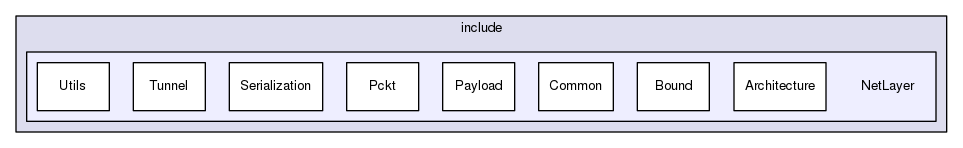
\includegraphics[width=0.85\textwidth]{inc/0.png}
\end{figure}

\begin{figure}[!htb]
\caption{NetLayer module dependencies.}
\centering
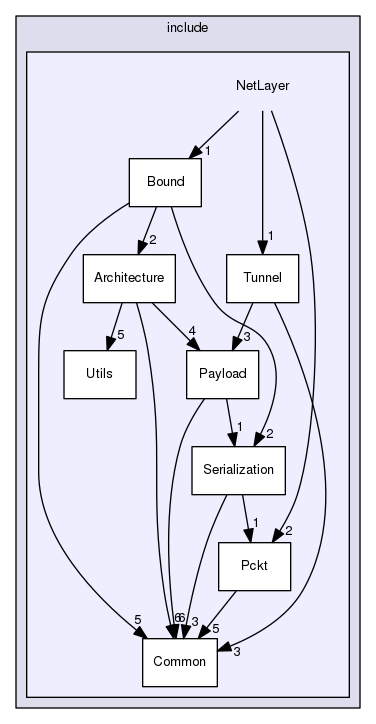
\includegraphics[width=0.35\textwidth]{inc/deps.png}
\end{figure}

\begin{figure}[!htb]
\caption{Serialization dependency graph.}
\centering
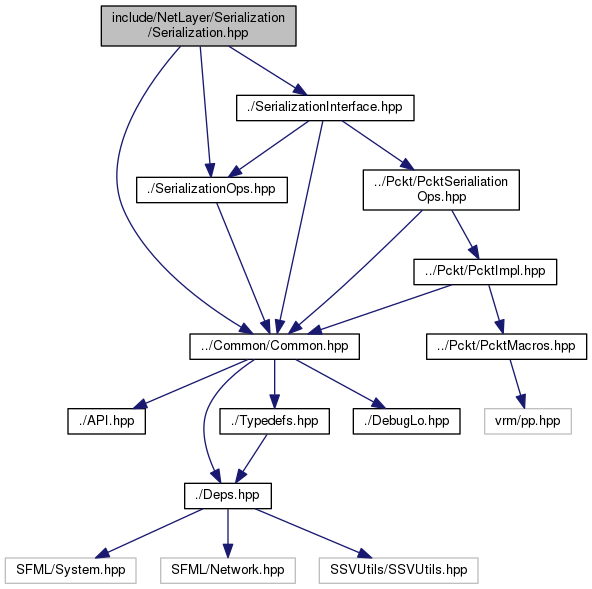
\includegraphics[width=0.9\textwidth]{inc/dep_ser.png}
\end{figure}

\begin{figure}[!htb]
\caption{Tunnel dependency graph.}
\centering
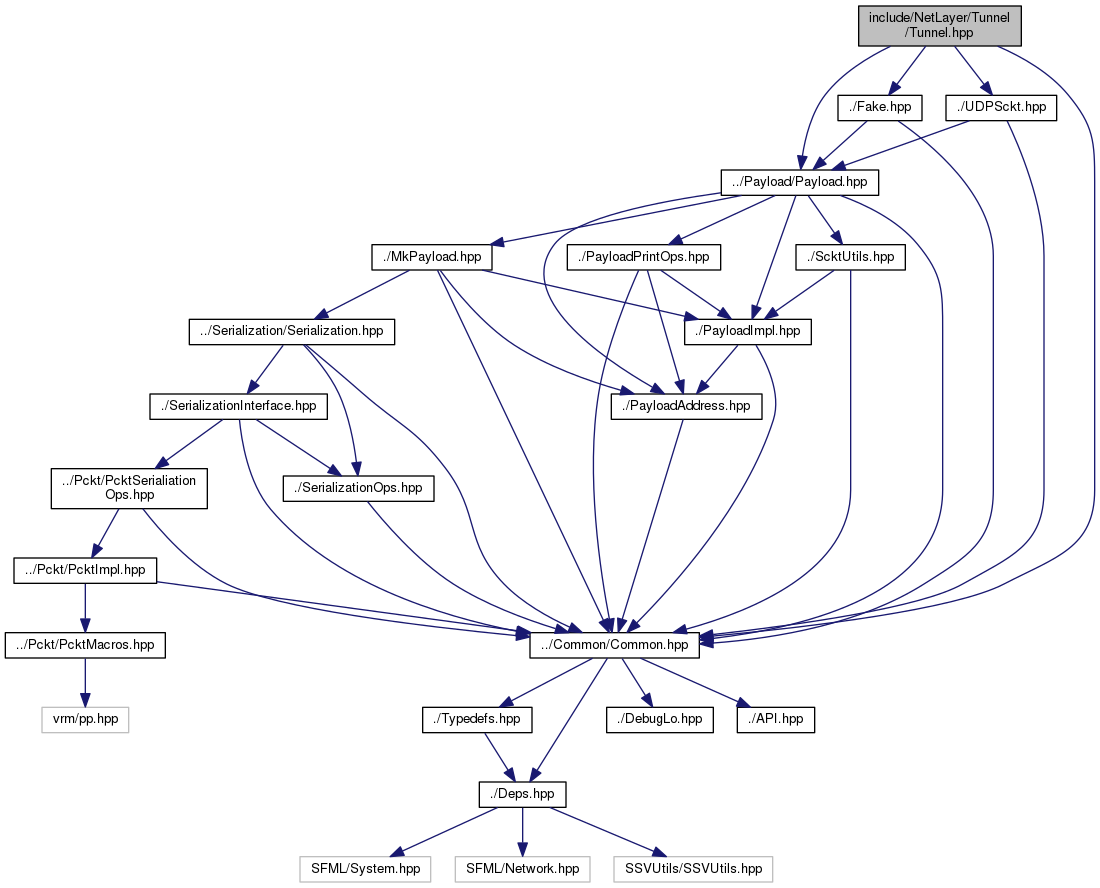
\includegraphics[width=1\textwidth]{inc/dep_tunnel.png}
\end{figure}

\begin{figure}[!htb]
\caption{Payload dependency graph.}
\centering
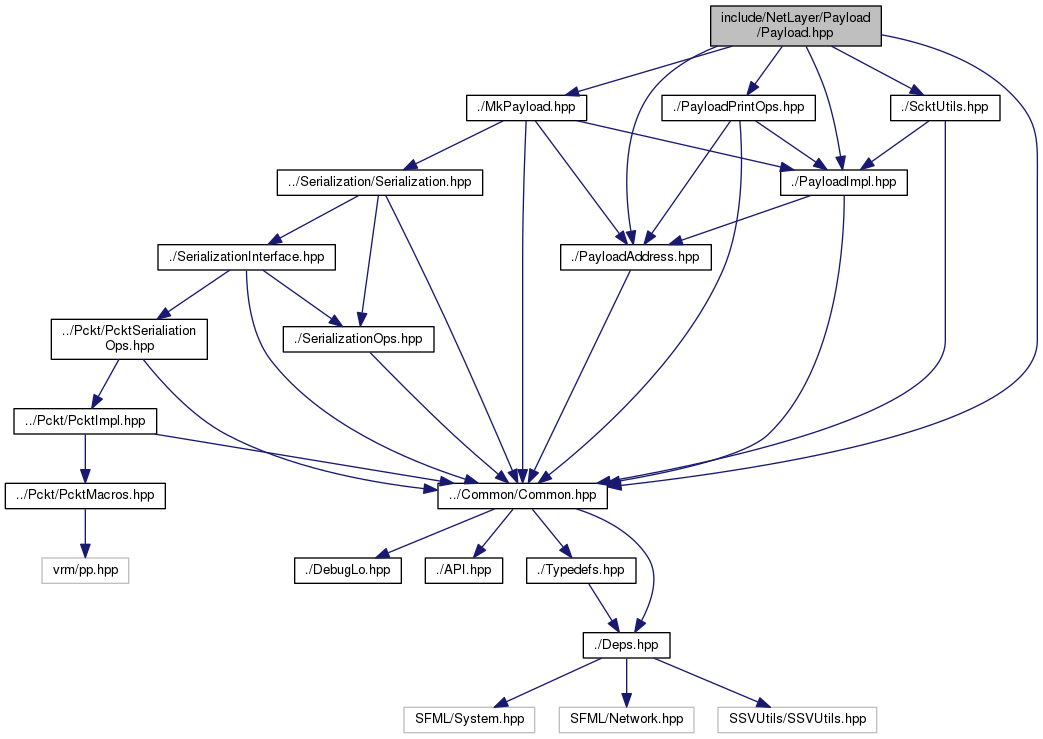
\includegraphics[width=1\textwidth]{inc/dep_paylod.png}
\end{figure}

\begin{figure}[!htb]
\caption{Packet types dependency graph.}
\centering
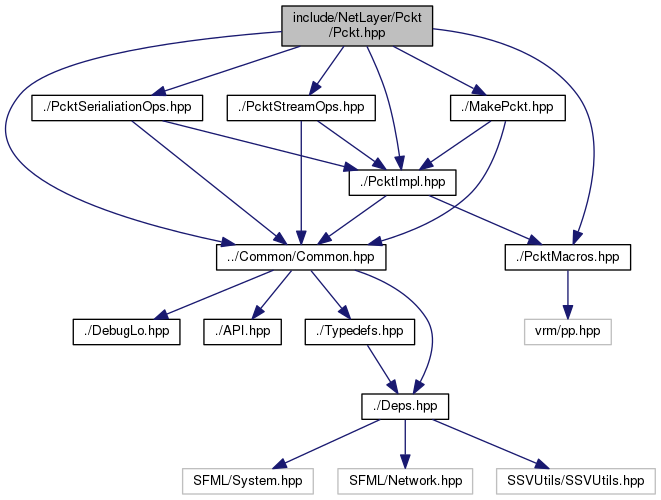
\includegraphics[width=0.95\textwidth]{inc/dep_pckt.png}
\end{figure}

\begin{figure}[!htb]
\caption{Architecture dependency graph.}
\centering
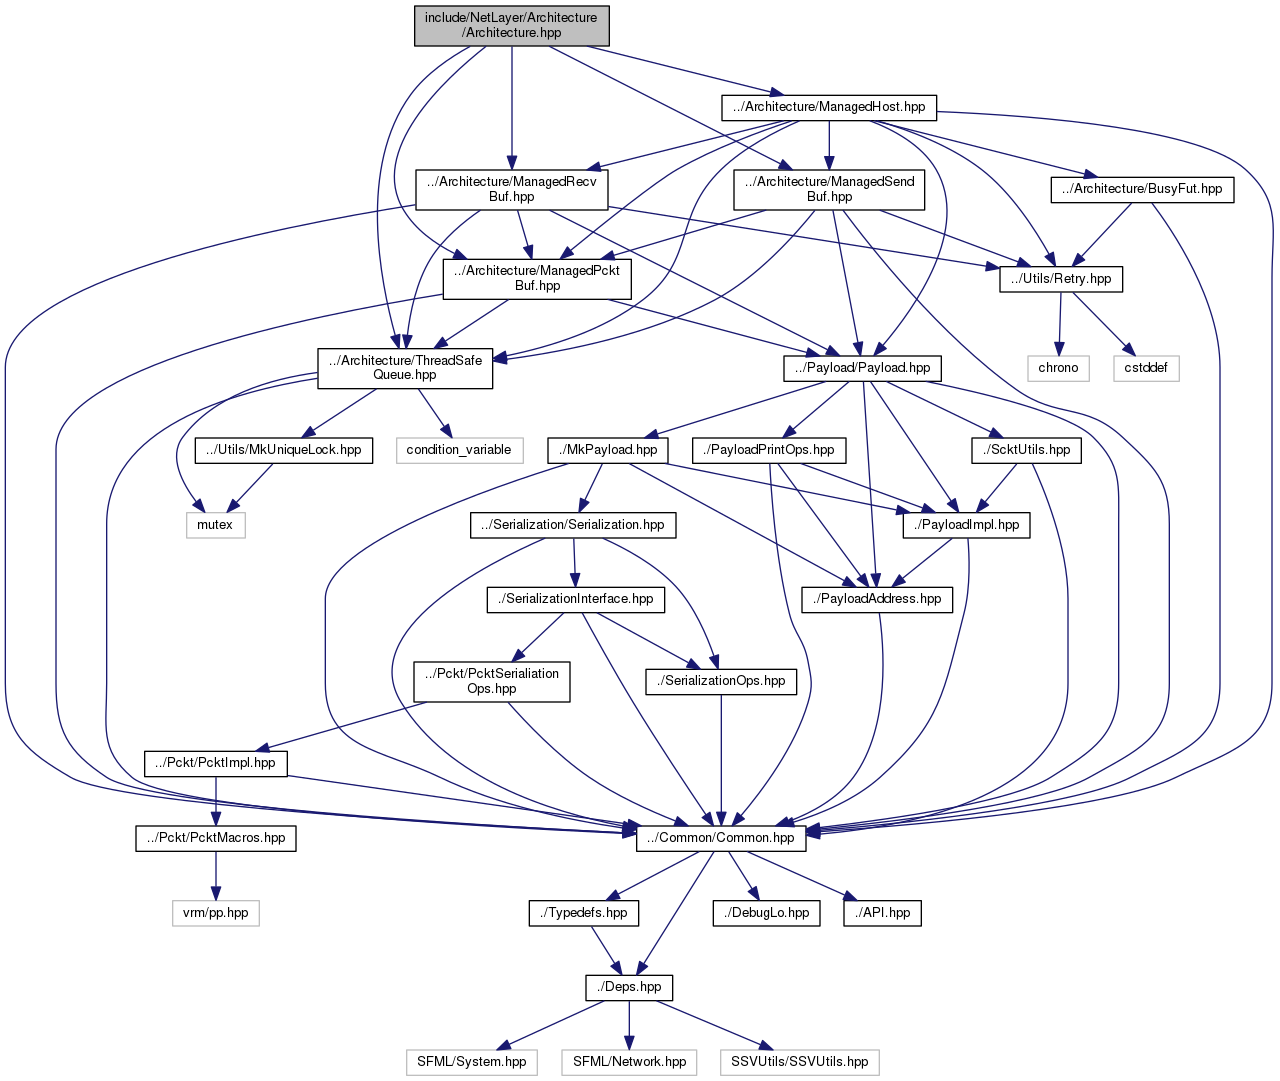
\includegraphics[width=1\textwidth]{inc/dep_archi.png}
\end{figure}

\chapter{Class documentation}
\hypertarget{classnl_1_1impl_1_1busy__loop}{}\section{nl\+:\+:impl\+:\+:busy\+\_\+loop Class Reference}
\label{classnl_1_1impl_1_1busy__loop}\index{nl\+::impl\+::busy\+\_\+loop@{nl\+::impl\+::busy\+\_\+loop}}


Wrapper around an {\ttfamily std\+::future$<$void$>$} that runs a busy loop until explicitly stopped by the user.  




{\ttfamily \#include $<$Busy\+Fut.\+hpp$>$}



Collaboration diagram for nl\+:\+:impl\+:\+:busy\+\_\+loop\+:\nopagebreak
\begin{figure}[H]
\begin{center}
\leavevmode
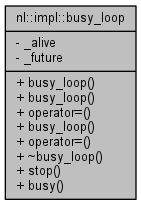
\includegraphics[width=178pt]{df/df6/classnl_1_1impl_1_1busy__loop__coll__graph}
\end{center}
\end{figure}
\subsection*{Public Member Functions}
\begin{DoxyCompactItemize}
\item 
\hypertarget{classnl_1_1impl_1_1busy__loop_aa90031dad092b534ad04f8b0a8d310fb}{}{\footnotesize template$<$typename T\+F $>$ }\\{\bfseries busy\+\_\+loop} (T\+F \&\&f)\label{classnl_1_1impl_1_1busy__loop_aa90031dad092b534ad04f8b0a8d310fb}

\item 
\hypertarget{classnl_1_1impl_1_1busy__loop_a00867955e79dea43ca66fd3169fd25b1}{}{\bfseries busy\+\_\+loop} (const \hyperlink{classnl_1_1impl_1_1busy__loop}{busy\+\_\+loop} \&)=delete\label{classnl_1_1impl_1_1busy__loop_a00867955e79dea43ca66fd3169fd25b1}

\item 
\hypertarget{classnl_1_1impl_1_1busy__loop_ac97e49816016b063bf3ded02a78ddc9a}{}\hyperlink{classnl_1_1impl_1_1busy__loop}{busy\+\_\+loop} \& {\bfseries operator=} (const \hyperlink{classnl_1_1impl_1_1busy__loop}{busy\+\_\+loop} \&)=delete\label{classnl_1_1impl_1_1busy__loop_ac97e49816016b063bf3ded02a78ddc9a}

\item 
\hypertarget{classnl_1_1impl_1_1busy__loop_ac11b40f801382e85a5f72d1184b35e02}{}{\bfseries busy\+\_\+loop} (\hyperlink{classnl_1_1impl_1_1busy__loop}{busy\+\_\+loop} \&\&)=default\label{classnl_1_1impl_1_1busy__loop_ac11b40f801382e85a5f72d1184b35e02}

\item 
\hypertarget{classnl_1_1impl_1_1busy__loop_a867ecb7a0829ecdd3d4ec36facee9056}{}\hyperlink{classnl_1_1impl_1_1busy__loop}{busy\+\_\+loop} \& {\bfseries operator=} (\hyperlink{classnl_1_1impl_1_1busy__loop}{busy\+\_\+loop} \&\&)=default\label{classnl_1_1impl_1_1busy__loop_a867ecb7a0829ecdd3d4ec36facee9056}

\item 
\hypertarget{classnl_1_1impl_1_1busy__loop_af0cca385fef844e8bca27da8e5462286}{}void {\bfseries stop} () noexcept\label{classnl_1_1impl_1_1busy__loop_af0cca385fef844e8bca27da8e5462286}

\item 
\hypertarget{classnl_1_1impl_1_1busy__loop_a71f36579b50a203cbc9d7730748bc4d1}{}bool {\bfseries busy} () const  noexcept\label{classnl_1_1impl_1_1busy__loop_a71f36579b50a203cbc9d7730748bc4d1}

\end{DoxyCompactItemize}


\subsection{Detailed Description}
Wrapper around an {\ttfamily std\+::future$<$void$>$} that runs a busy loop until explicitly stopped by the user. 

The documentation for this class was generated from the following file\+:\begin{DoxyCompactItemize}
\item 
include/\+Net\+Layer/\+Architecture/Busy\+Fut.\+hpp\end{DoxyCompactItemize}

%\hypertarget{structexperiment_1_1Config}{}\section{experiment\+:\+:Config$<$ T\+Settings, T\+Bind\+List $>$ Struct Template Reference}
\label{structexperiment_1_1Config}\index{experiment\+::\+Config$<$ T\+Settings, T\+Bind\+List $>$@{experiment\+::\+Config$<$ T\+Settings, T\+Bind\+List $>$}}


Collaboration diagram for experiment\+:\+:Config$<$ T\+Settings, T\+Bind\+List $>$\+:\nopagebreak
\begin{figure}[H]
\begin{center}
\leavevmode
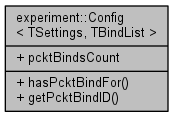
\includegraphics[width=204pt]{d5/d13/structexperiment_1_1Config__coll__graph}
\end{center}
\end{figure}
\subsection*{Public Types}
\begin{DoxyCompactItemize}
\item 
\hypertarget{structexperiment_1_1Config_a96431f152cbf395d1072a953b9cbebbd}{}using {\bfseries I\+D\+Type} = typename T\+Settings\+::\+I\+D\+Type\label{structexperiment_1_1Config_a96431f152cbf395d1072a953b9cbebbd}

\item 
\hypertarget{structexperiment_1_1Config_a6fd649e27ccccdb8aff35cee3cb331aa}{}using {\bfseries Settings} = T\+Settings\label{structexperiment_1_1Config_a6fd649e27ccccdb8aff35cee3cb331aa}

\item 
\hypertarget{structexperiment_1_1Config_a80a051a9b92ba43f95bd555fa2b0c038}{}using {\bfseries Pckt\+Binds} = T\+Bind\+List\label{structexperiment_1_1Config_a80a051a9b92ba43f95bd555fa2b0c038}

\end{DoxyCompactItemize}
\subsection*{Static Public Member Functions}
\begin{DoxyCompactItemize}
\item 
\hypertarget{structexperiment_1_1Config_a2980bcb1deb87a1572e76c9da19845ce}{}{\footnotesize template$<$typename T $>$ }\\static constexpr auto {\bfseries has\+Pckt\+Bind\+For} () noexcept\label{structexperiment_1_1Config_a2980bcb1deb87a1572e76c9da19845ce}

\item 
\hypertarget{structexperiment_1_1Config_ad62e6c85c77cb2bf5abd2c20f73ef483}{}{\footnotesize template$<$typename T $>$ }\\static constexpr auto {\bfseries get\+Pckt\+Bind\+I\+D} () noexcept\label{structexperiment_1_1Config_ad62e6c85c77cb2bf5abd2c20f73ef483}

\end{DoxyCompactItemize}
\subsection*{Static Public Attributes}
\begin{DoxyCompactItemize}
\item 
\hypertarget{structexperiment_1_1Config_a4cf90d96b9f16ce019cc71a75d5b7f9a}{}static constexpr std\+::size\+\_\+t {\bfseries pckt\+Binds\+Count} \{M\+P\+L\+::size$<$Pckt\+Binds$>$()\}\label{structexperiment_1_1Config_a4cf90d96b9f16ce019cc71a75d5b7f9a}

\end{DoxyCompactItemize}


The documentation for this struct was generated from the following file\+:\begin{DoxyCompactItemize}
\item 
include/\+Net\+Layer/\+Bound/Config.\+hpp\end{DoxyCompactItemize}

\hypertarget{classexperiment_1_1ContextHost}{}\section{experiment\+:\+:Context\+Host$<$ T\+Config $>$ Class Template Reference}
\label{classexperiment_1_1ContextHost}\index{experiment\+::\+Context\+Host$<$ T\+Config $>$@{experiment\+::\+Context\+Host$<$ T\+Config $>$}}


Collaboration diagram for experiment\+:\+:Context\+Host$<$ T\+Config $>$\+:\nopagebreak
\begin{figure}[H]
\begin{center}
\leavevmode
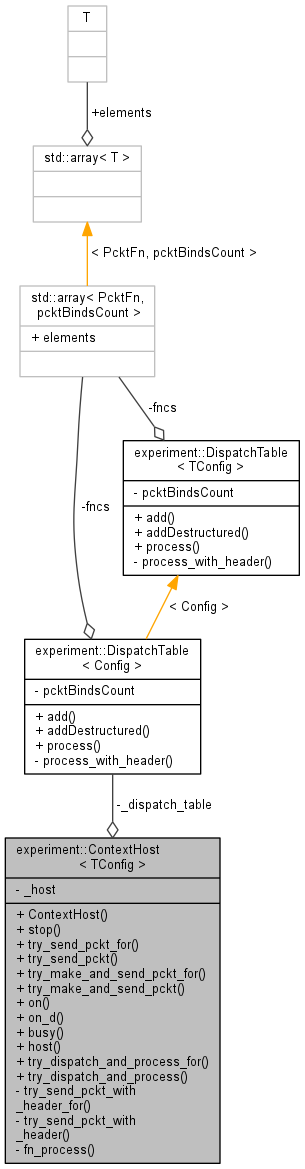
\includegraphics[width=242pt]{d9/d53/classexperiment_1_1ContextHost__coll__graph}
\end{center}
\end{figure}
\subsection*{Public Member Functions}
\begin{DoxyCompactItemize}
\item 
\hypertarget{classexperiment_1_1ContextHost_adb4f5d162ffadfc8a01e92a7679921c4}{}{\bfseries Context\+Host} (nl\+::\+Port port)\label{classexperiment_1_1ContextHost_adb4f5d162ffadfc8a01e92a7679921c4}

\item 
\hypertarget{classexperiment_1_1ContextHost_a7b81799a5f49ec088426ea6828b13cb5}{}void {\bfseries stop} ()\label{classexperiment_1_1ContextHost_a7b81799a5f49ec088426ea6828b13cb5}

\item 
\hypertarget{classexperiment_1_1ContextHost_a81478849fd6be0e3a9e477315640612a}{}{\footnotesize template$<$typename T , typename T\+Duration $>$ }\\auto {\bfseries try\+\_\+send\+\_\+pckt\+\_\+for} (const \hyperlink{structnl_1_1PAddress}{P\+Address} \&pa, const T\+Duration \&d, T \&\&pckt)\label{classexperiment_1_1ContextHost_a81478849fd6be0e3a9e477315640612a}

\item 
\hypertarget{classexperiment_1_1ContextHost_a104dd3085b47ee168da8448e6b0a2c16}{}{\footnotesize template$<$typename T $>$ }\\auto {\bfseries try\+\_\+send\+\_\+pckt} (const \hyperlink{structnl_1_1PAddress}{P\+Address} \&pa, T \&\&pckt)\label{classexperiment_1_1ContextHost_a104dd3085b47ee168da8448e6b0a2c16}

\item 
\hypertarget{classexperiment_1_1ContextHost_ac0e1482bcd559dd01965f2d0b08565a6}{}{\footnotesize template$<$typename T , typename T\+Duration , typename... Ts$>$ }\\auto {\bfseries try\+\_\+make\+\_\+and\+\_\+send\+\_\+pckt\+\_\+for} (const \hyperlink{structnl_1_1PAddress}{P\+Address} \&pa, const T\+Duration \&d, Ts \&\&...xs)\label{classexperiment_1_1ContextHost_ac0e1482bcd559dd01965f2d0b08565a6}

\item 
\hypertarget{classexperiment_1_1ContextHost_ad65ee5e4fe93f7110070ec7a0ce6f8fb}{}{\footnotesize template$<$typename T , typename... Ts$>$ }\\auto {\bfseries try\+\_\+make\+\_\+and\+\_\+send\+\_\+pckt} (const \hyperlink{structnl_1_1PAddress}{P\+Address} \&pa, Ts \&\&...xs)\label{classexperiment_1_1ContextHost_ad65ee5e4fe93f7110070ec7a0ce6f8fb}

\item 
\hypertarget{classexperiment_1_1ContextHost_a30edc8ffb1bdbc07e90e46990fba4f04}{}{\footnotesize template$<$typename T\+Pckt , typename T\+F $>$ }\\void {\bfseries on} (T\+F \&\&fn)\label{classexperiment_1_1ContextHost_a30edc8ffb1bdbc07e90e46990fba4f04}

\item 
\hypertarget{classexperiment_1_1ContextHost_a95781cbfbf975455ae1dec256e8f329a}{}{\footnotesize template$<$typename T\+Pckt , typename T\+F $>$ }\\void {\bfseries on\+\_\+d} (T\+F \&\&fn)\label{classexperiment_1_1ContextHost_a95781cbfbf975455ae1dec256e8f329a}

\item 
\hypertarget{classexperiment_1_1ContextHost_afb39c3ebae58dcd5aa8afc8346814dc3}{}bool {\bfseries busy} () const  noexcept\label{classexperiment_1_1ContextHost_afb39c3ebae58dcd5aa8afc8346814dc3}

\item 
\hypertarget{classexperiment_1_1ContextHost_aef94042a8ad58227d4b1a0ae7be4ff62}{}auto \& {\bfseries host} () noexcept\label{classexperiment_1_1ContextHost_aef94042a8ad58227d4b1a0ae7be4ff62}

\item 
\hypertarget{classexperiment_1_1ContextHost_a2fe68c36c9fc33fbd9e821606ebbc28c}{}{\footnotesize template$<$typename T\+Duration $>$ }\\auto {\bfseries try\+\_\+dispatch\+\_\+and\+\_\+process\+\_\+for} (const T\+Duration \&d)\label{classexperiment_1_1ContextHost_a2fe68c36c9fc33fbd9e821606ebbc28c}

\item 
\hypertarget{classexperiment_1_1ContextHost_a41af40283cb5c0152e912b94e925e074}{}auto {\bfseries try\+\_\+dispatch\+\_\+and\+\_\+process} ()\label{classexperiment_1_1ContextHost_a41af40283cb5c0152e912b94e925e074}

\end{DoxyCompactItemize}


The documentation for this class was generated from the following file\+:\begin{DoxyCompactItemize}
\item 
include/\+Net\+Layer/\+Bound/Context\+Host.\+hpp\end{DoxyCompactItemize}

\hypertarget{classexperiment_1_1DispatchTable}{}\section{experiment\+:\+:Dispatch\+Table$<$ T\+Config $>$ Class Template Reference}
\label{classexperiment_1_1DispatchTable}\index{experiment\+::\+Dispatch\+Table$<$ T\+Config $>$@{experiment\+::\+Dispatch\+Table$<$ T\+Config $>$}}


Inheritance diagram for experiment\+:\+:Dispatch\+Table$<$ T\+Config $>$\+:\nopagebreak
\begin{figure}[H]
\begin{center}
\leavevmode
\includegraphics[width=214pt]{d1/dcb/classexperiment_1_1DispatchTable__inherit__graph}
\end{center}
\end{figure}


Collaboration diagram for experiment\+:\+:Dispatch\+Table$<$ T\+Config $>$\+:\nopagebreak
\begin{figure}[H]
\begin{center}
\leavevmode
\includegraphics[width=214pt]{d7/d4e/classexperiment_1_1DispatchTable__coll__graph}
\end{center}
\end{figure}
\subsection*{Public Member Functions}
\begin{DoxyCompactItemize}
\item 
\hypertarget{classexperiment_1_1DispatchTable_a84002d58d9223f5677be1212eb947005}{}{\footnotesize template$<$typename T , typename T\+F $>$ }\\void {\bfseries add} (T\+F \&\&fn\+To\+Call)\label{classexperiment_1_1DispatchTable_a84002d58d9223f5677be1212eb947005}

\item 
\hypertarget{classexperiment_1_1DispatchTable_a31966af1468a06b7b669fdff141cb2d6}{}{\footnotesize template$<$typename T , typename T\+F $>$ }\\void {\bfseries add\+Destructured} (T\+F \&\&fn\+To\+Call)\label{classexperiment_1_1DispatchTable_a31966af1468a06b7b669fdff141cb2d6}

\item 
\hypertarget{classexperiment_1_1DispatchTable_a28107f8398ff02447afd291180b38331}{}void {\bfseries process} (const \hyperlink{structnl_1_1PAddress}{P\+Address} \&sender, Pckt\+Buf \&p)\label{classexperiment_1_1DispatchTable_a28107f8398ff02447afd291180b38331}

\end{DoxyCompactItemize}


The documentation for this class was generated from the following file\+:\begin{DoxyCompactItemize}
\item 
include/\+Net\+Layer/\+Bound/Dispatch\+Table.\+hpp\end{DoxyCompactItemize}

%\hypertarget{structnl_1_1impl_1_1Tunnel_1_1Fake}{}\section{nl\+:\+:impl\+:\+:Tunnel\+:\+:Fake Struct Reference}
\label{structnl_1_1impl_1_1Tunnel_1_1Fake}\index{nl\+::impl\+::\+Tunnel\+::\+Fake@{nl\+::impl\+::\+Tunnel\+::\+Fake}}


Collaboration diagram for nl\+:\+:impl\+:\+:Tunnel\+:\+:Fake\+:\nopagebreak
\begin{figure}[H]
\begin{center}
\leavevmode
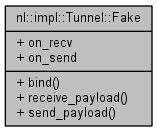
\includegraphics[width=191pt]{d3/d92/structnl_1_1impl_1_1Tunnel_1_1Fake__coll__graph}
\end{center}
\end{figure}
\subsection*{Public Member Functions}
\begin{DoxyCompactItemize}
\item 
\hypertarget{structnl_1_1impl_1_1Tunnel_1_1Fake_a3e463ac8462d8cd4fabc669a68c0aab0}{}bool {\bfseries bind} (Port)\label{structnl_1_1impl_1_1Tunnel_1_1Fake_a3e463ac8462d8cd4fabc669a68c0aab0}

\item 
\hypertarget{structnl_1_1impl_1_1Tunnel_1_1Fake_a86ecf7e0ea1c99b7ed926a5c057661d1}{}auto {\bfseries receive\+\_\+payload} (\hyperlink{structnl_1_1Payload}{Payload} \&p)\label{structnl_1_1impl_1_1Tunnel_1_1Fake_a86ecf7e0ea1c99b7ed926a5c057661d1}

\item 
\hypertarget{structnl_1_1impl_1_1Tunnel_1_1Fake_a2c6f5a3406a0c13b5ed86306130af8bc}{}auto {\bfseries send\+\_\+payload} (\hyperlink{structnl_1_1Payload}{Payload} \&p)\label{structnl_1_1impl_1_1Tunnel_1_1Fake_a2c6f5a3406a0c13b5ed86306130af8bc}

\end{DoxyCompactItemize}
\subsection*{Public Attributes}
\begin{DoxyCompactItemize}
\item 
\hypertarget{structnl_1_1impl_1_1Tunnel_1_1Fake_a804a29756a339f3b65f33988b5f5cf40}{}std\+::function$<$ void(\hyperlink{structnl_1_1Payload}{Payload} \&)$>$ {\bfseries on\+\_\+recv}\label{structnl_1_1impl_1_1Tunnel_1_1Fake_a804a29756a339f3b65f33988b5f5cf40}

\item 
\hypertarget{structnl_1_1impl_1_1Tunnel_1_1Fake_a271b065b4864c762ee029881e8acccb4}{}std\+::function$<$ void(\hyperlink{structnl_1_1Payload}{Payload} \&)$>$ {\bfseries on\+\_\+send}\label{structnl_1_1impl_1_1Tunnel_1_1Fake_a271b065b4864c762ee029881e8acccb4}

\end{DoxyCompactItemize}


The documentation for this struct was generated from the following file\+:\begin{DoxyCompactItemize}
\item 
include/\+Net\+Layer/\+Tunnel/Fake.\+hpp\end{DoxyCompactItemize}

%\hypertarget{structnl_1_1init__fields}{}\section{nl\+:\+:init\+\_\+fields Struct Reference}
\label{structnl_1_1init__fields}\index{nl\+::init\+\_\+fields@{nl\+::init\+\_\+fields}}


Collaboration diagram for nl\+:\+:init\+\_\+fields\+:\nopagebreak
\begin{figure}[H]
\begin{center}
\leavevmode
\includegraphics[width=151pt]{dc/d51/structnl_1_1init__fields__coll__graph}
\end{center}
\end{figure}


The documentation for this struct was generated from the following file\+:\begin{DoxyCompactItemize}
\item 
include/\+Net\+Layer/\+Pckt/Pckt\+Impl.\+hpp\end{DoxyCompactItemize}

\hypertarget{classnl_1_1ManagedHostImpl}{}\section{nl\+:\+:Managed\+Host\+Impl$<$ T\+Tunnel $>$ Class Template Reference}
\label{classnl_1_1ManagedHostImpl}\index{nl\+::\+Managed\+Host\+Impl$<$ T\+Tunnel $>$@{nl\+::\+Managed\+Host\+Impl$<$ T\+Tunnel $>$}}


Collaboration diagram for nl\+:\+:Managed\+Host\+Impl$<$ T\+Tunnel $>$\+:\nopagebreak
\begin{figure}[H]
\begin{center}
\leavevmode
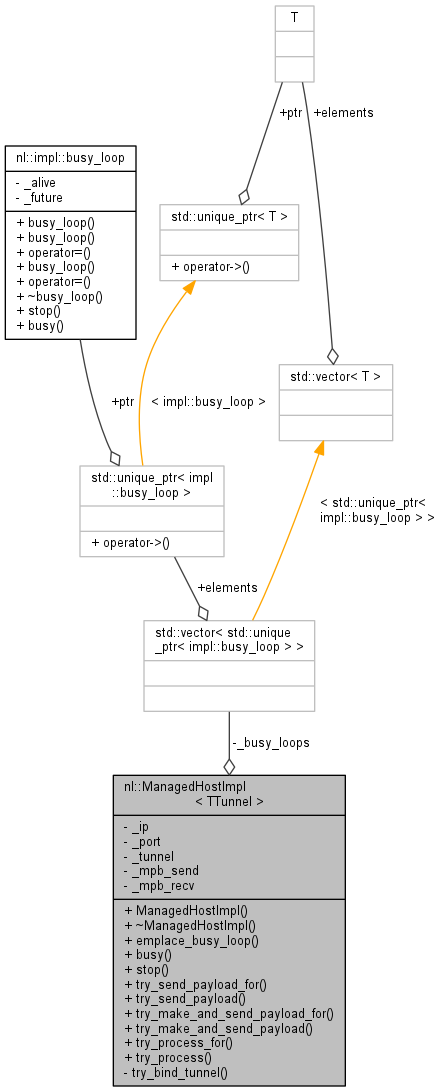
\includegraphics[width=255pt]{d5/dfb/classnl_1_1ManagedHostImpl__coll__graph}
\end{center}
\end{figure}
\subsection*{Public Member Functions}
\begin{DoxyCompactItemize}
\item 
\hypertarget{classnl_1_1ManagedHostImpl_aef1cdf80463dd1a9690ef03e088c1d66}{}{\footnotesize template$<$typename... T\+Tunnel\+Args$>$ }\\{\bfseries Managed\+Host\+Impl} (Port port, T\+Tunnel\+Args \&\&...ts)\label{classnl_1_1ManagedHostImpl_aef1cdf80463dd1a9690ef03e088c1d66}

\item 
\hypertarget{classnl_1_1ManagedHostImpl_a626bc07441217d08e475560869d7a023}{}{\footnotesize template$<$typename T\+F $>$ }\\auto \& {\bfseries emplace\+\_\+busy\+\_\+loop} (T\+F \&\&f)\label{classnl_1_1ManagedHostImpl_a626bc07441217d08e475560869d7a023}

\item 
\hypertarget{classnl_1_1ManagedHostImpl_ac412d63b60ee98d9c14da8c6688a1712}{}bool {\bfseries busy} () const  noexcept\label{classnl_1_1ManagedHostImpl_ac412d63b60ee98d9c14da8c6688a1712}

\item 
\hypertarget{classnl_1_1ManagedHostImpl_a202ff37cc7bcc9d7711361ccf50ec3bc}{}void {\bfseries stop} ()\label{classnl_1_1ManagedHostImpl_a202ff37cc7bcc9d7711361ccf50ec3bc}

\item 
\hypertarget{classnl_1_1ManagedHostImpl_a94ead799412e023175e9fbadf5251e9c}{}{\footnotesize template$<$typename T\+Duration $>$ }\\auto {\bfseries try\+\_\+send\+\_\+payload\+\_\+for} (\hyperlink{structnl_1_1Payload}{Payload} \&p, const T\+Duration \&d)\label{classnl_1_1ManagedHostImpl_a94ead799412e023175e9fbadf5251e9c}

\item 
\hypertarget{classnl_1_1ManagedHostImpl_affcbc6cb0fba53b4a388ef256008a7d2}{}auto {\bfseries try\+\_\+send\+\_\+payload} (\hyperlink{structnl_1_1Payload}{Payload} \&p)\label{classnl_1_1ManagedHostImpl_affcbc6cb0fba53b4a388ef256008a7d2}

\item 
\hypertarget{classnl_1_1ManagedHostImpl_a6436ffecc416447858a378d10a2f4653}{}{\footnotesize template$<$typename T\+Duration , typename... Ts$>$ }\\auto {\bfseries try\+\_\+make\+\_\+and\+\_\+send\+\_\+payload\+\_\+for} (const \hyperlink{structnl_1_1PAddress}{P\+Address} \&pa, const T\+Duration \&d, Ts \&\&...xs)\label{classnl_1_1ManagedHostImpl_a6436ffecc416447858a378d10a2f4653}

\item 
\hypertarget{classnl_1_1ManagedHostImpl_aef1bc53fa9e1f37cf5b0f2842c5babd9}{}{\footnotesize template$<$typename... Ts$>$ }\\auto {\bfseries try\+\_\+make\+\_\+and\+\_\+send\+\_\+payload} (const \hyperlink{structnl_1_1PAddress}{P\+Address} \&pa, Ts \&\&...xs)\label{classnl_1_1ManagedHostImpl_aef1bc53fa9e1f37cf5b0f2842c5babd9}

\item 
\hypertarget{classnl_1_1ManagedHostImpl_a9db9147845f2abccd4a2a24b55322ede}{}{\footnotesize template$<$typename T\+F , typename T\+Duration $>$ }\\bool {\bfseries try\+\_\+process\+\_\+for} (const T\+Duration \&d, T\+F \&\&f)\label{classnl_1_1ManagedHostImpl_a9db9147845f2abccd4a2a24b55322ede}

\item 
\hypertarget{classnl_1_1ManagedHostImpl_ae3b7955e15c744e5bcc4851730e6152d}{}{\footnotesize template$<$typename T\+F $>$ }\\bool {\bfseries try\+\_\+process} (T\+F \&\&f)\label{classnl_1_1ManagedHostImpl_ae3b7955e15c744e5bcc4851730e6152d}

\end{DoxyCompactItemize}


The documentation for this class was generated from the following file\+:\begin{DoxyCompactItemize}
\item 
include/\+Net\+Layer/\+Architecture/Managed\+Host.\+hpp\end{DoxyCompactItemize}

\hypertarget{classnl_1_1impl_1_1ManagedPcktBuf}{}\section{nl\+:\+:impl\+:\+:Managed\+Pckt\+Buf$<$ T\+Tunnel $>$ Class Template Reference}
\label{classnl_1_1impl_1_1ManagedPcktBuf}\index{nl\+::impl\+::\+Managed\+Pckt\+Buf$<$ T\+Tunnel $>$@{nl\+::impl\+::\+Managed\+Pckt\+Buf$<$ T\+Tunnel $>$}}


Inheritance diagram for nl\+:\+:impl\+:\+:Managed\+Pckt\+Buf$<$ T\+Tunnel $>$\+:\nopagebreak
\begin{figure}[H]
\begin{center}
\leavevmode
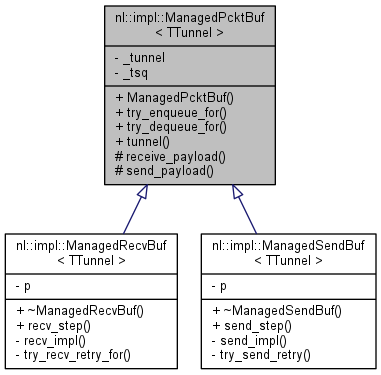
\includegraphics[width=350pt]{df/d90/classnl_1_1impl_1_1ManagedPcktBuf__inherit__graph}
\end{center}
\end{figure}


Collaboration diagram for nl\+:\+:impl\+:\+:Managed\+Pckt\+Buf$<$ T\+Tunnel $>$\+:\nopagebreak
\begin{figure}[H]
\begin{center}
\leavevmode
\includegraphics[width=209pt]{d0/d14/classnl_1_1impl_1_1ManagedPcktBuf__coll__graph}
\end{center}
\end{figure}
\subsection*{Public Member Functions}
\begin{DoxyCompactItemize}
\item 
\hypertarget{classnl_1_1impl_1_1ManagedPcktBuf_a26972960cfcd62151dd87f246b960dfd}{}{\bfseries Managed\+Pckt\+Buf} (T\+Tunnel \&t)\label{classnl_1_1impl_1_1ManagedPcktBuf_a26972960cfcd62151dd87f246b960dfd}

\item 
\hypertarget{classnl_1_1impl_1_1ManagedPcktBuf_a2bf2f583f806a1d0ee3946d6c75353ef}{}{\footnotesize template$<$typename T\+Duration , typename... Ts$>$ }\\bool {\bfseries try\+\_\+enqueue\+\_\+for} (const T\+Duration \&d, Ts \&\&...xs)\label{classnl_1_1impl_1_1ManagedPcktBuf_a2bf2f583f806a1d0ee3946d6c75353ef}

\item 
\hypertarget{classnl_1_1impl_1_1ManagedPcktBuf_ad6c6576b99b53107ebb548a907610178}{}{\footnotesize template$<$typename T\+Duration $>$ }\\bool {\bfseries try\+\_\+dequeue\+\_\+for} (const T\+Duration \&d, \hyperlink{structnl_1_1Payload}{Payload} \&p)\label{classnl_1_1impl_1_1ManagedPcktBuf_ad6c6576b99b53107ebb548a907610178}

\item 
\hypertarget{classnl_1_1impl_1_1ManagedPcktBuf_a3cd3f076d0729eb11e74b26401822cee}{}auto \& {\bfseries tunnel} () noexcept\label{classnl_1_1impl_1_1ManagedPcktBuf_a3cd3f076d0729eb11e74b26401822cee}

\end{DoxyCompactItemize}
\subsection*{Protected Member Functions}
\begin{DoxyCompactItemize}
\item 
\hypertarget{classnl_1_1impl_1_1ManagedPcktBuf_a1e28a6735c585548b8277b5544101d3f}{}auto {\bfseries receive\+\_\+payload} (\hyperlink{structnl_1_1Payload}{Payload} \&p)\label{classnl_1_1impl_1_1ManagedPcktBuf_a1e28a6735c585548b8277b5544101d3f}

\item 
\hypertarget{classnl_1_1impl_1_1ManagedPcktBuf_a16cb9aa8f9c0153f0a6af9bc352161ec}{}auto {\bfseries send\+\_\+payload} (\hyperlink{structnl_1_1Payload}{Payload} \&p)\label{classnl_1_1impl_1_1ManagedPcktBuf_a16cb9aa8f9c0153f0a6af9bc352161ec}

\end{DoxyCompactItemize}


The documentation for this class was generated from the following file\+:\begin{DoxyCompactItemize}
\item 
include/\+Net\+Layer/\+Architecture/Managed\+Pckt\+Buf.\+hpp\end{DoxyCompactItemize}

\hypertarget{classnl_1_1impl_1_1ManagedRecvBuf}{}\section{nl\+:\+:impl\+:\+:Managed\+Recv\+Buf$<$ T\+Tunnel $>$ Class Template Reference}
\label{classnl_1_1impl_1_1ManagedRecvBuf}\index{nl\+::impl\+::\+Managed\+Recv\+Buf$<$ T\+Tunnel $>$@{nl\+::impl\+::\+Managed\+Recv\+Buf$<$ T\+Tunnel $>$}}


Inheritance diagram for nl\+:\+:impl\+:\+:Managed\+Recv\+Buf$<$ T\+Tunnel $>$\+:\nopagebreak
\begin{figure}[H]
\begin{center}
\leavevmode
\includegraphics[width=212pt]{de/d2c/classnl_1_1impl_1_1ManagedRecvBuf__inherit__graph}
\end{center}
\end{figure}


Collaboration diagram for nl\+:\+:impl\+:\+:Managed\+Recv\+Buf$<$ T\+Tunnel $>$\+:\nopagebreak
\begin{figure}[H]
\begin{center}
\leavevmode
\includegraphics[width=212pt]{da/d22/classnl_1_1impl_1_1ManagedRecvBuf__coll__graph}
\end{center}
\end{figure}
\subsection*{Public Member Functions}
\begin{DoxyCompactItemize}
\item 
\hypertarget{classnl_1_1impl_1_1ManagedRecvBuf_a0ea2535503e7c1116ccbee2c501c813a}{}auto {\bfseries recv\+\_\+step} ()\label{classnl_1_1impl_1_1ManagedRecvBuf_a0ea2535503e7c1116ccbee2c501c813a}

\end{DoxyCompactItemize}
\subsection*{Additional Inherited Members}


The documentation for this class was generated from the following file\+:\begin{DoxyCompactItemize}
\item 
include/\+Net\+Layer/\+Architecture/Managed\+Recv\+Buf.\+hpp\end{DoxyCompactItemize}

\hypertarget{classnl_1_1impl_1_1ManagedSendBuf}{}\section{nl\+:\+:impl\+:\+:Managed\+Send\+Buf$<$ T\+Tunnel $>$ Class Template Reference}
\label{classnl_1_1impl_1_1ManagedSendBuf}\index{nl\+::impl\+::\+Managed\+Send\+Buf$<$ T\+Tunnel $>$@{nl\+::impl\+::\+Managed\+Send\+Buf$<$ T\+Tunnel $>$}}


Inheritance diagram for nl\+:\+:impl\+:\+:Managed\+Send\+Buf$<$ T\+Tunnel $>$\+:\nopagebreak
\begin{figure}[H]
\begin{center}
\leavevmode
\includegraphics[width=211pt]{dd/d80/classnl_1_1impl_1_1ManagedSendBuf__inherit__graph}
\end{center}
\end{figure}


Collaboration diagram for nl\+:\+:impl\+:\+:Managed\+Send\+Buf$<$ T\+Tunnel $>$\+:\nopagebreak
\begin{figure}[H]
\begin{center}
\leavevmode
\includegraphics[width=211pt]{d5/d80/classnl_1_1impl_1_1ManagedSendBuf__coll__graph}
\end{center}
\end{figure}
\subsection*{Public Member Functions}
\begin{DoxyCompactItemize}
\item 
\hypertarget{classnl_1_1impl_1_1ManagedSendBuf_a07d7f60b6c6ac190283ad3e1c7fed896}{}auto {\bfseries send\+\_\+step} ()\label{classnl_1_1impl_1_1ManagedSendBuf_a07d7f60b6c6ac190283ad3e1c7fed896}

\end{DoxyCompactItemize}
\subsection*{Additional Inherited Members}


The documentation for this class was generated from the following file\+:\begin{DoxyCompactItemize}
\item 
include/\+Net\+Layer/\+Architecture/Managed\+Send\+Buf.\+hpp\end{DoxyCompactItemize}

\hypertarget{structnl_1_1PAddress}{}\section{nl\+:\+:P\+Address Struct Reference}
\label{structnl_1_1PAddress}\index{nl\+::\+P\+Address@{nl\+::\+P\+Address}}


Collaboration diagram for nl\+:\+:P\+Address\+:\nopagebreak
\begin{figure}[H]
\begin{center}
\leavevmode
\includegraphics[width=159pt]{d0/da4/structnl_1_1PAddress__coll__graph}
\end{center}
\end{figure}
\subsection*{Public Member Functions}
\begin{DoxyCompactItemize}
\item 
\hypertarget{structnl_1_1PAddress_a3b3d447ae6ae2e5214269c87207c646d}{}{\bfseries P\+Address} (const Ip\+Addr \&m\+Ip, Port m\+Port) noexcept\label{structnl_1_1PAddress_a3b3d447ae6ae2e5214269c87207c646d}

\item 
\hypertarget{structnl_1_1PAddress_aa906da75ec8f742ba39e46937f90dac0}{}bool {\bfseries operator==} (const \hyperlink{structnl_1_1PAddress}{P\+Address} \&rhs) const  noexcept\label{structnl_1_1PAddress_aa906da75ec8f742ba39e46937f90dac0}

\item 
\hypertarget{structnl_1_1PAddress_abed553d216e8203324d5e1d65b79a38f}{}bool {\bfseries operator!=} (const \hyperlink{structnl_1_1PAddress}{P\+Address} \&rhs) const  noexcept\label{structnl_1_1PAddress_abed553d216e8203324d5e1d65b79a38f}

\item 
\hypertarget{structnl_1_1PAddress_ab3e5b075669c046ab457932288bb8ec3}{}bool {\bfseries operator$<$} (const \hyperlink{structnl_1_1PAddress}{P\+Address} \&rhs) const  noexcept\label{structnl_1_1PAddress_ab3e5b075669c046ab457932288bb8ec3}

\end{DoxyCompactItemize}
\subsection*{Public Attributes}
\begin{DoxyCompactItemize}
\item 
\hypertarget{structnl_1_1PAddress_a997be42c475a48bdaca279d6c267ff8f}{}Ip\+Addr {\bfseries ip}\label{structnl_1_1PAddress_a997be42c475a48bdaca279d6c267ff8f}

\item 
\hypertarget{structnl_1_1PAddress_ac7a3e4ddc831aa22676ecd7b7e6041ee}{}Port {\bfseries port}\label{structnl_1_1PAddress_ac7a3e4ddc831aa22676ecd7b7e6041ee}

\end{DoxyCompactItemize}


The documentation for this struct was generated from the following file\+:\begin{DoxyCompactItemize}
\item 
include/\+Net\+Layer/\+Payload/Payload\+Address.\+hpp\end{DoxyCompactItemize}

\hypertarget{structnl_1_1Payload}{}\section{nl\+:\+:Payload Struct Reference}
\label{structnl_1_1Payload}\index{nl\+::\+Payload@{nl\+::\+Payload}}


Collaboration diagram for nl\+:\+:Payload\+:\nopagebreak
\begin{figure}[H]
\begin{center}
\leavevmode
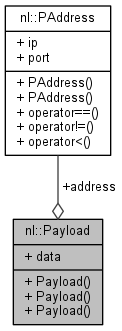
\includegraphics[width=164pt]{dd/d5f/structnl_1_1Payload__coll__graph}
\end{center}
\end{figure}
\subsection*{Public Member Functions}
\begin{DoxyCompactItemize}
\item 
\hypertarget{structnl_1_1Payload_a69fdb72c6756252c3d3dae312caf97ae}{}{\bfseries Payload} (const \hyperlink{structnl_1_1PAddress}{P\+Address} \&m\+Address) noexcept\label{structnl_1_1Payload_a69fdb72c6756252c3d3dae312caf97ae}

\item 
\hypertarget{structnl_1_1Payload_a83d1e4e02369b17f3f1ddfa85c1f4823}{}{\footnotesize template$<$typename T\+Data $>$ }\\{\bfseries Payload} (const \hyperlink{structnl_1_1PAddress}{P\+Address} \&m\+Address, T\+Data \&\&m\+Data)\label{structnl_1_1Payload_a83d1e4e02369b17f3f1ddfa85c1f4823}

\end{DoxyCompactItemize}
\subsection*{Public Attributes}
\begin{DoxyCompactItemize}
\item 
\hypertarget{structnl_1_1Payload_a5cd9e5b5e6271123bf564ac5fb8e4971}{}\hyperlink{structnl_1_1PAddress}{P\+Address} {\bfseries address}\label{structnl_1_1Payload_a5cd9e5b5e6271123bf564ac5fb8e4971}

\item 
\hypertarget{structnl_1_1Payload_aa5d03839f17a000d8a333352a29180be}{}Pckt\+Buf {\bfseries data}\label{structnl_1_1Payload_aa5d03839f17a000d8a333352a29180be}

\end{DoxyCompactItemize}


The documentation for this struct was generated from the following file\+:\begin{DoxyCompactItemize}
\item 
include/\+Net\+Layer/\+Payload/Payload\+Impl.\+hpp\end{DoxyCompactItemize}

\hypertarget{structnl_1_1impl_1_1Pckt}{}\section{nl\+:\+:impl\+:\+:Pckt$<$ T\+Fields $>$ Struct Template Reference}
\label{structnl_1_1impl_1_1Pckt}\index{nl\+::impl\+::\+Pckt$<$ T\+Fields $>$@{nl\+::impl\+::\+Pckt$<$ T\+Fields $>$}}


Inheritance diagram for nl\+:\+:impl\+:\+:Pckt$<$ T\+Fields $>$\+:\nopagebreak
\begin{figure}[H]
\begin{center}
\leavevmode
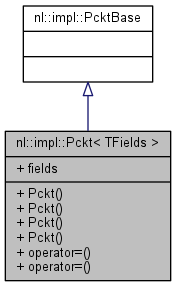
\includegraphics[width=205pt]{de/d52/structnl_1_1impl_1_1Pckt__inherit__graph}
\end{center}
\end{figure}


Collaboration diagram for nl\+:\+:impl\+:\+:Pckt$<$ T\+Fields $>$\+:\nopagebreak
\begin{figure}[H]
\begin{center}
\leavevmode
\includegraphics[width=205pt]{de/d2f/structnl_1_1impl_1_1Pckt__coll__graph}
\end{center}
\end{figure}
\subsection*{Public Types}
\begin{DoxyCompactItemize}
\item 
\hypertarget{structnl_1_1impl_1_1Pckt_a68f3f720d95233652c169c971e271d8a}{}using {\bfseries Tpl\+Type} = std\+::tuple$<$ T\+Fields... $>$\label{structnl_1_1impl_1_1Pckt_a68f3f720d95233652c169c971e271d8a}

\end{DoxyCompactItemize}
\subsection*{Public Member Functions}
\begin{DoxyCompactItemize}
\item 
\hypertarget{structnl_1_1impl_1_1Pckt_a40beeef4aa8d787f714779139f13e525}{}{\footnotesize template$<$typename... Ts$>$ }\\{\bfseries Pckt} (\hyperlink{structnl_1_1init__fields}{nl\+::init\+\_\+fields}, Ts \&\&...m\+X)\label{structnl_1_1impl_1_1Pckt_a40beeef4aa8d787f714779139f13e525}

\item 
\hypertarget{structnl_1_1impl_1_1Pckt_a192a758292a9f2477fc26c3c6362a5e6}{}{\bfseries Pckt} (const \hyperlink{structnl_1_1impl_1_1Pckt}{Pckt} \&m\+X)\label{structnl_1_1impl_1_1Pckt_a192a758292a9f2477fc26c3c6362a5e6}

\item 
\hypertarget{structnl_1_1impl_1_1Pckt_a027967cfeb8de8ccfb78b641b38fcbaa}{}{\bfseries Pckt} (\hyperlink{structnl_1_1impl_1_1Pckt}{Pckt} \&\&m\+X)\label{structnl_1_1impl_1_1Pckt_a027967cfeb8de8ccfb78b641b38fcbaa}

\item 
\hypertarget{structnl_1_1impl_1_1Pckt_a7f4b332d332e5bbcb03a539b9486b314}{}\hyperlink{structnl_1_1impl_1_1Pckt}{Pckt} \& {\bfseries operator=} (const \hyperlink{structnl_1_1impl_1_1Pckt}{Pckt} \&m\+X)\label{structnl_1_1impl_1_1Pckt_a7f4b332d332e5bbcb03a539b9486b314}

\item 
\hypertarget{structnl_1_1impl_1_1Pckt_acb484b18d906024bd251c4ab8d057923}{}\hyperlink{structnl_1_1impl_1_1Pckt}{Pckt} \& {\bfseries operator=} (\hyperlink{structnl_1_1impl_1_1Pckt}{Pckt} \&\&m\+X)\label{structnl_1_1impl_1_1Pckt_acb484b18d906024bd251c4ab8d057923}

\end{DoxyCompactItemize}
\subsection*{Public Attributes}
\begin{DoxyCompactItemize}
\item 
\hypertarget{structnl_1_1impl_1_1Pckt_a2ac6777ba49d071e03c3413b9d023212}{}Tpl\+Type {\bfseries fields}\label{structnl_1_1impl_1_1Pckt_a2ac6777ba49d071e03c3413b9d023212}

\end{DoxyCompactItemize}


The documentation for this struct was generated from the following file\+:\begin{DoxyCompactItemize}
\item 
include/\+Net\+Layer/\+Pckt/Pckt\+Impl.\+hpp\end{DoxyCompactItemize}

%\hypertarget{structexperiment_1_1impl_1_1pckt__bind__type}{}\section{experiment\+:\+:impl\+:\+:pckt\+\_\+bind\+\_\+type$<$ T $>$ Struct Template Reference}
\label{structexperiment_1_1impl_1_1pckt__bind__type}\index{experiment\+::impl\+::pckt\+\_\+bind\+\_\+type$<$ T $>$@{experiment\+::impl\+::pckt\+\_\+bind\+\_\+type$<$ T $>$}}


Collaboration diagram for experiment\+:\+:impl\+:\+:pckt\+\_\+bind\+\_\+type$<$ T $>$\+:\nopagebreak
\begin{figure}[H]
\begin{center}
\leavevmode
\includegraphics[width=193pt]{d9/d14/structexperiment_1_1impl_1_1pckt__bind__type__coll__graph}
\end{center}
\end{figure}
\subsection*{Public Types}
\begin{DoxyCompactItemize}
\item 
\hypertarget{structexperiment_1_1impl_1_1pckt__bind__type_a29ef06f11cc6f45c50ead44f7cf0cfb5}{}using {\bfseries type} = T\label{structexperiment_1_1impl_1_1pckt__bind__type_a29ef06f11cc6f45c50ead44f7cf0cfb5}

\end{DoxyCompactItemize}


The documentation for this struct was generated from the following file\+:\begin{DoxyCompactItemize}
\item 
include/\+Net\+Layer/\+Bound/Pckt\+Bind.\+hpp\end{DoxyCompactItemize}

%\hypertarget{structnl_1_1impl_1_1PcktBase}{}\section{nl\+:\+:impl\+:\+:Pckt\+Base Struct Reference}
\label{structnl_1_1impl_1_1PcktBase}\index{nl\+::impl\+::\+Pckt\+Base@{nl\+::impl\+::\+Pckt\+Base}}


Inheritance diagram for nl\+:\+:impl\+:\+:Pckt\+Base\+:\nopagebreak
\begin{figure}[H]
\begin{center}
\leavevmode
\includegraphics[width=205pt]{d1/d75/structnl_1_1impl_1_1PcktBase__inherit__graph}
\end{center}
\end{figure}


Collaboration diagram for nl\+:\+:impl\+:\+:Pckt\+Base\+:\nopagebreak
\begin{figure}[H]
\begin{center}
\leavevmode
\includegraphics[width=177pt]{d9/d51/structnl_1_1impl_1_1PcktBase__coll__graph}
\end{center}
\end{figure}


The documentation for this struct was generated from the following file\+:\begin{DoxyCompactItemize}
\item 
include/\+Net\+Layer/\+Pckt/Pckt\+Impl.\+hpp\end{DoxyCompactItemize}

%\hypertarget{structexperiment_1_1Settings}{}\section{experiment\+:\+:Settings$<$ T\+I\+D\+Type $>$ Struct Template Reference}
\label{structexperiment_1_1Settings}\index{experiment\+::\+Settings$<$ T\+I\+D\+Type $>$@{experiment\+::\+Settings$<$ T\+I\+D\+Type $>$}}


Collaboration diagram for experiment\+:\+:Settings$<$ T\+I\+D\+Type $>$\+:\nopagebreak
\begin{figure}[H]
\begin{center}
\leavevmode
\includegraphics[width=187pt]{d7/de2/structexperiment_1_1Settings__coll__graph}
\end{center}
\end{figure}
\subsection*{Public Types}
\begin{DoxyCompactItemize}
\item 
\hypertarget{structexperiment_1_1Settings_a464b29ad8283cfb1404054398a23852c}{}using {\bfseries I\+D\+Type} = T\+I\+D\+Type\label{structexperiment_1_1Settings_a464b29ad8283cfb1404054398a23852c}

\end{DoxyCompactItemize}


The documentation for this struct was generated from the following file\+:\begin{DoxyCompactItemize}
\item 
include/\+Net\+Layer/\+Bound/Settings.\+hpp\end{DoxyCompactItemize}

\hypertarget{classnl_1_1impl_1_1ThreadSafeQueue}{}\section{nl\+:\+:impl\+:\+:Thread\+Safe\+Queue$<$ T $>$ Class Template Reference}
\label{classnl_1_1impl_1_1ThreadSafeQueue}\index{nl\+::impl\+::\+Thread\+Safe\+Queue$<$ T $>$@{nl\+::impl\+::\+Thread\+Safe\+Queue$<$ T $>$}}


Inheritance diagram for nl\+:\+:impl\+:\+:Thread\+Safe\+Queue$<$ T $>$\+:\nopagebreak
\begin{figure}[H]
\begin{center}
\leavevmode
\includegraphics[width=237pt]{d8/d51/classnl_1_1impl_1_1ThreadSafeQueue__inherit__graph}
\end{center}
\end{figure}


Collaboration diagram for nl\+:\+:impl\+:\+:Thread\+Safe\+Queue$<$ T $>$\+:\nopagebreak
\begin{figure}[H]
\begin{center}
\leavevmode
\includegraphics[width=237pt]{d5/d4d/classnl_1_1impl_1_1ThreadSafeQueue__coll__graph}
\end{center}
\end{figure}
\subsection*{Public Member Functions}
\begin{DoxyCompactItemize}
\item 
\hypertarget{classnl_1_1impl_1_1ThreadSafeQueue_aba290c00615c2a3d7226ece08139fa9d}{}{\footnotesize template$<$typename... T\+Args$>$ }\\void {\bfseries enqueue} (T\+Args \&\&...m\+Args)\label{classnl_1_1impl_1_1ThreadSafeQueue_aba290c00615c2a3d7226ece08139fa9d}

\item 
\hypertarget{classnl_1_1impl_1_1ThreadSafeQueue_a63e740704fd67c4eeb1a1539db3a92dd}{}{\footnotesize template$<$typename T\+Duration , typename... T\+Args$>$ }\\bool {\bfseries try\+\_\+enqueue\+\_\+for} (const T\+Duration \&m\+Duration, T\+Args \&\&...m\+Args)\label{classnl_1_1impl_1_1ThreadSafeQueue_a63e740704fd67c4eeb1a1539db3a92dd}

\item 
\hypertarget{classnl_1_1impl_1_1ThreadSafeQueue_a7e6eb4c05f8e58219d4890f2de418d40}{}T {\bfseries dequeue} ()\label{classnl_1_1impl_1_1ThreadSafeQueue_a7e6eb4c05f8e58219d4890f2de418d40}

\item 
\hypertarget{classnl_1_1impl_1_1ThreadSafeQueue_a99ec655141bbafed60b6d15c8fdfd6e8}{}{\footnotesize template$<$typename T\+Duration $>$ }\\bool {\bfseries try\+\_\+dequeue\+\_\+for} (const T\+Duration \&m\+Duration, T \&m\+Out)\label{classnl_1_1impl_1_1ThreadSafeQueue_a99ec655141bbafed60b6d15c8fdfd6e8}

\item 
\hypertarget{classnl_1_1impl_1_1ThreadSafeQueue_a6b308dfe4c501bba96fd8506a1d88010}{}auto {\bfseries size} () const \label{classnl_1_1impl_1_1ThreadSafeQueue_a6b308dfe4c501bba96fd8506a1d88010}

\item 
\hypertarget{classnl_1_1impl_1_1ThreadSafeQueue_a9aa3cf7fb8ebdc816dc6104e41aa81f0}{}auto {\bfseries empty} () const \label{classnl_1_1impl_1_1ThreadSafeQueue_a9aa3cf7fb8ebdc816dc6104e41aa81f0}

\end{DoxyCompactItemize}


The documentation for this class was generated from the following file\+:\begin{DoxyCompactItemize}
\item 
include/\+Net\+Layer/\+Architecture/Thread\+Safe\+Queue.\+hpp\end{DoxyCompactItemize}

\hypertarget{classnl_1_1impl_1_1Tunnel_1_1UDPSckt}{}\section{nl\+:\+:impl\+:\+:Tunnel\+:\+:U\+D\+P\+Sckt Class Reference}
\label{classnl_1_1impl_1_1Tunnel_1_1UDPSckt}\index{nl\+::impl\+::\+Tunnel\+::\+U\+D\+P\+Sckt@{nl\+::impl\+::\+Tunnel\+::\+U\+D\+P\+Sckt}}


Collaboration diagram for nl\+:\+:impl\+:\+:Tunnel\+:\+:U\+D\+P\+Sckt\+:\nopagebreak
\begin{figure}[H]
\begin{center}
\leavevmode
\includegraphics[width=211pt]{d3/d04/classnl_1_1impl_1_1Tunnel_1_1UDPSckt__coll__graph}
\end{center}
\end{figure}
\subsection*{Public Member Functions}
\begin{DoxyCompactItemize}
\item 
\hypertarget{classnl_1_1impl_1_1Tunnel_1_1UDPSckt_a051b9d00d5833099efb0a0b7e0a56d56}{}{\bfseries U\+D\+P\+Sckt} (const \hyperlink{classnl_1_1impl_1_1Tunnel_1_1UDPSckt}{U\+D\+P\+Sckt} \&)=delete\label{classnl_1_1impl_1_1Tunnel_1_1UDPSckt_a051b9d00d5833099efb0a0b7e0a56d56}

\item 
\hypertarget{classnl_1_1impl_1_1Tunnel_1_1UDPSckt_a44b657ca44acf2dd756a7bae3466663a}{}\hyperlink{classnl_1_1impl_1_1Tunnel_1_1UDPSckt}{U\+D\+P\+Sckt} \& {\bfseries operator=} (const \hyperlink{classnl_1_1impl_1_1Tunnel_1_1UDPSckt}{U\+D\+P\+Sckt} \&)=delete\label{classnl_1_1impl_1_1Tunnel_1_1UDPSckt_a44b657ca44acf2dd756a7bae3466663a}

\item 
\hypertarget{classnl_1_1impl_1_1Tunnel_1_1UDPSckt_ae0bd9188147ac27bf69eb97196ed7227}{}{\bfseries U\+D\+P\+Sckt} (\hyperlink{classnl_1_1impl_1_1Tunnel_1_1UDPSckt}{U\+D\+P\+Sckt} \&\&)=default\label{classnl_1_1impl_1_1Tunnel_1_1UDPSckt_ae0bd9188147ac27bf69eb97196ed7227}

\item 
\hypertarget{classnl_1_1impl_1_1Tunnel_1_1UDPSckt_a6be403baed83c611195278f0061d5fc8}{}\hyperlink{classnl_1_1impl_1_1Tunnel_1_1UDPSckt}{U\+D\+P\+Sckt} \& {\bfseries operator=} (\hyperlink{classnl_1_1impl_1_1Tunnel_1_1UDPSckt}{U\+D\+P\+Sckt} \&\&)=default\label{classnl_1_1impl_1_1Tunnel_1_1UDPSckt_a6be403baed83c611195278f0061d5fc8}

\item 
\hypertarget{classnl_1_1impl_1_1Tunnel_1_1UDPSckt_a7cf869256058fe18b96e92605b2b73b0}{}{\footnotesize template$<$typename... Ts$>$ }\\{\bfseries U\+D\+P\+Sckt} (Ts \&\&...xs)\label{classnl_1_1impl_1_1Tunnel_1_1UDPSckt_a7cf869256058fe18b96e92605b2b73b0}

\item 
\hypertarget{classnl_1_1impl_1_1Tunnel_1_1UDPSckt_adb9b8dcfd4cab068d3d8a88009c00546}{}bool {\bfseries bind} (Port x)\label{classnl_1_1impl_1_1Tunnel_1_1UDPSckt_adb9b8dcfd4cab068d3d8a88009c00546}

\item 
\hypertarget{classnl_1_1impl_1_1Tunnel_1_1UDPSckt_af7b8e61ba4fc3e3b0200328677d57c42}{}auto {\bfseries receive\+\_\+payload} (\hyperlink{structnl_1_1Payload}{Payload} \&p)\label{classnl_1_1impl_1_1Tunnel_1_1UDPSckt_af7b8e61ba4fc3e3b0200328677d57c42}

\item 
\hypertarget{classnl_1_1impl_1_1Tunnel_1_1UDPSckt_adf830eb3a290fb5eb3b6e7aabbbe1f44}{}auto {\bfseries send\+\_\+payload} (\hyperlink{structnl_1_1Payload}{Payload} \&p)\label{classnl_1_1impl_1_1Tunnel_1_1UDPSckt_adf830eb3a290fb5eb3b6e7aabbbe1f44}

\end{DoxyCompactItemize}


The documentation for this class was generated from the following file\+:\begin{DoxyCompactItemize}
\item 
include/\+Net\+Layer/\+Tunnel/U\+D\+P\+Sckt.\+hpp\end{DoxyCompactItemize}




\end{document}




